\documentclass[12pt]{report}% Šablona Kristiāns Kacars 2022. Last updated 08.02.2023

%\usepackage[utf8]{inputenc} neizmanto XeLatex, tad jāatkomentē.
\usepackage[T1]{fontenc}
\usepackage{geometry}
\geometry{
 a4paper,
 left=30mm,
 top=20mm,
 right=20mm,
 bottom=20mm,
 includefoot
 }


\usepackage{xcolor}
\usepackage[]{graphicx}
\usepackage{setspace}
%\onehalfspacing %rindstarpas 1.5 vienības
\linespread{1.5}
\usepackage{placeins}%ērti izmantot \FloatBarrier, lai neļauti attēliem aiziet pārāk tālu no vajadzīgās vietas.
\usepackage{titlesec}%izveido atstarpes starp chapter un section nosaukumu
\usepackage{indentfirst}%pirmai rindkopai sekcijas sākumā nav atkāpe, ar šo tā tiek uzlikta
\titleformat{\chapter}
  {\normalfont\fontsize{16}{18}\bfseries\raggedright}{\thechapter.}{0pt}{\MakeUppercase}{}
  
\titleformat{\section}
  {\normalfont\fontsize{14}{16}\bfseries}{\thesection}{1em}{}
\titleformat{\subsection}
  {\normalfont\fontsize{12}{16}\bfseries}{\thesubsection}{1em}{}  

\titlespacing*{\chapter}{0pt}{0pt}{10pt}
\titlespacing*{\section}{0pt}{5pt}{5pt}


% \usepackage{fancyhdr}%šis izveido header, lai tur ir līnija ar section nosaukumu
% \newcommand{\changefont}{%
%     \fontsize{9}{11}\selectfont
% }
% \pagestyle{fancy}
% \fancyhf{}
% \fancyfoot[C]{\thepage}
% \fancyhead[L]{\changefont \leftmark}

\usepackage{polyglossia}
\setdefaultlanguage{latvian}
\usepackage{lipsum}
\setlength{\parskip}{1.5pt}%atstarpe starp rindkopām

%matematikas paketes
\usepackage{amsmath} 
\usepackage{amsthm}
\usepackage{amssymb}
\usepackage{bm}%ērts priekš treknraksta matemātiskajā vidē
\usepackage{esint}%integrāļu zīmes, kas nav parastajās ams paketēs

%--pašizveidotās matemātikas komandas
\newcommand{\bra}{\langle}
\newcommand{\ket}{\rangle}
%--

\newtheorem{theorem}{Teorēma}
\theoremstyle{definition}
\newtheorem{definition}{Definīcija}

\usepackage{siunitx}%mērvienībām


%Algoritmu atspoguļošanai
\usepackage[ruled, vlined, linesnumbered, algochapter]{algorithm2e}
\renewcommand{\algorithmcfname}{Algoritms}% nomaina nosaukumu uz latviešu variantu
\usepackage[labelfont={bf}]{caption}%attēlu un tabulu nosaukumu fonts

\usepackage[style=phys,%der arī citi, piem., chem-angew(bibliogrāfijā pie article nav links)
articletitle=false,
biblabel=brackets,%
chaptertitle=false,%
    sorting=none,%kārto pēc citēšanas secības
    date=short]{biblatex}
\addbibresource{biblio.bib}

% normalizēts formatējums atsaucēm
\DeclareFieldFormat*{title}{\textnormal{#1}}
\DeclareFieldFormat*{journaltitle}{\textnormal{#1}}
\DeclareFieldFormat*{booktitle}{\textnormal{#1}}
\DeclareFieldFormat{url}{\textnormal{\url{#1}}}
\AtEveryBibitem{\normalfont}

\usepackage{hyperref}%Izveido spiežamus linkus saturam, bibliogrāfijām uc.
\hypersetup{
    colorlinks,
    citecolor=blue,
    filecolor=black,
    linkcolor=black,
    urlcolor=black
}


\newcommand*{\SavedEqref}{}%Dod krāsainus un spiežamus vienādojumu linkus
\let\SavedEqref\eqref
\renewcommand*{\eqref}[1]{%
  \begingroup
    \hypersetup{
      linkcolor=blue,
      linkbordercolor=black,
    }%
    \SavedEqref{#1}%
  \endgroup
}%vienādojumiem


\usepackage{chngcntr}%figure numeration
\counterwithin{figure}{chapter}
\counterwithin{table}{chapter}
\counterwithin{equation}{chapter}%vienadojumu numerācija veidojas pa nodaļām



%Pakete izveido apzīmējumu sarakstu
\usepackage{nomencl}
\makenomenclature
\renewcommand{\nomname}{Apzīmējumu saraksts}
%% Sadala grupās apzīmējumus
%Ja gribat pievienot papildu kategoriju, nokopējat-->
%   \ifstrequal{#1}{F}{Fizikas konstantes}{%
% tikai pēdējā rindiņā( kur ir Lielumu apzīmējumi) ieliekat papildu "}"
% -----------------------------------------
\usepackage{etoolbox}
\renewcommand\nomgroup[1]{%
  \item[\bfseries
  \ifstrequal{#1}{N}{}
]}

% pakete priekš koda formatēšanas
\usepackage{listings}
\renewcommand{\lstlistingname}{Izdruka}
\lstset{
  language=C++,
  basicstyle=\ttfamily\small,
  keywordstyle=\color{blue},
  stringstyle=\color{red},
  commentstyle=\color{green!50!black},
  numbers=left,
  numberstyle=\tiny\color{gray},
  stepnumber=1,
  frame=single,
  tabsize=2,
  breaklines=true,
  showstringspaces=false,
  aboveskip=1mm, % Reduce space above the listing
  belowskip=1mm, % Reduce space below the listing
  lineskip=-1pt, % Adjust line spacing between lines
}

\usepackage{tabularx}
\usepackage{tikz}
\usepackage{float}




% --------------------------------------------
% ------- beidzas package izsaukšana un stila veidošana






%%%--------- Aizpildīt titullapu---------- 
%% Šis aizpildīs template titullapu ar jūsu informāciju
% Darba tips, i.e. bakalaura vai maģistra
\def\degree{Kursa darbs}
% Fakultātes nosaukums
\def\faculty{Eksakto zinātņu un tehnoloģiju fakultāte}
% Nodaļa iekš fakultātes
\def\department{Datorikas nodaļa}
% Universitātes nosaukums
\def\university{Latvijas Universitāte}
% Universitātes logo
\def\crest{\includegraphics[width = 0.5\textwidth]{LU_logo_LV_horiz.png}}%ja ieliekat attēlu kādā mapē, tad jāsauc attēls no šīs mapes, citādi neparādīsies tas titullapā.
\def\vietlaiks{Rīga, 2024}
\def\supervisor{Darba vadītājs: profesors, Dr. dat. Leo Seļāvo}
\def\studaplieciba{ak21373}
\author{Artūrs Kļaviņš}
\title{GPU programmēšanas salīdzinājums CUDA, ROCm un OpenCL saskarnēs}
\date{Maijs 2025}
\newcommand{\thedate}[0]{01.05.2025}%iesniegšanas datums
%%%---------- Beidz aizpildīt titullapu----------- 




\begin{document}



\thispagestyle{empty}
\makeatletter
   \begin{center}
       \vspace*{1cm}
        
    \vspace{10mm}
    {\Large LATVIJAS UNIVERSITĀTE\\
    \MakeUppercase{\faculty}\\
    \vspace{2mm}
    \MakeUppercase{\department}
    }
    \vspace*{10mm}
    
    
    
    \vspace{5mm}
    {\Large \MakeUppercase{\textbf{\@title}}}
    \vspace{5mm}
    

       \vspace{1cm}
    \Large
    \MakeUppercase{\degree}
    \end{center}
    \vspace{3cm}
    \begin{flushleft}
    \large
       Autors: \textbf{\large \@author}\\
       Studenta apliecības Nr.: \studaplieciba \\
       \supervisor
    \end{flushleft}

       \vfill
     
    \begin{center}
    \Large      
    \MakeUppercase{\vietlaiks}
   \end{center}
\makeatother

\newpage




\thispagestyle{empty}
\noindent \textbf{Anotācija}

\noindent Darbā gan teorētiski, gan praktiski tiks apskatītas CUDA, ROCm un OpenCL GPU
programmēšanas saskarnes. Tiks salīdzināta saskarņu dokumentācija, piedāvātās
programmatūras iespējas un ierobežojumi atbalstītajā aparatūrā. Praktiski tiks ieviesta
paroļu uzlaušanas un Džona Konveja dzīves spēles programmas katrā saskarnē,
apskatīti īstenošanas apsvērumi un analizēta ātrdarbība uz vienas un tās pašas
aparatūras.

\vspace{4mm}
\noindent \textbf{Atslēgas vārdi}: GPU, Nvidia, AMD, CUDA, ROCm, OpenCL

\vspace{20mm}
\noindent \textbf{Abstract}

\noindent Abstract body

\vspace{4mm}
\noindent \textbf{Keywords}: GPU, Nvidia, AMD, CUDA, ROCm

\newpage
\tableofcontents
\newpage

%Apzīmējumu saraksts

\nomenclature[N]{GPU}{Grafiskais procesors (no angļu val. \textit{Graphical Processing Unit})}
\nomenclature[N]{CPU}{Centrālais procesors (no angļu val. \textit{Central Processing Unit})}
\nomenclature[N]{CUDA}{\textit{Compute Unified Device Architecture} ir Nvidia ieviests API, kas ļauj
programmatūrai izmantot NVIDIA ražotos GPU}
\nomenclature[N]{GPGPU}{\textit{General-purpose computing on graphics processing units} - plašlietojama
skaitļošana uz grafiskajiem procesoriem, mūsdienās ņem vērā un ievieš procesora arhitektūras līmenī}
\nomenclature[N]{Ēnotājs}{Datorgrafikas programma, kura apstrādā tekstūru, 3D objektu un ainu gaismas
līmeņus un krāsas}
\nomenclature[N]{HPC}{Augstas veiktspējas skaitļošana (no angļu val. \textit{High-performance Computing})
ir datoru klāsteru izmantošana, lai ar lielu paralelitātes pakāpi risinātu kādu problēmu, apstrādātu milzīga
apjoma datus}
\nomenclature[N]{ROCm}{AMD izstrādātā atvērtā pirmkoda platforma priekš HPC un AI darbiem ar videokartēm}
\nomenclature[N]{HIP}{ROCm sastāvdaļa, C++ API programmu izstrādei uz AMD un Nvidia videokartēm
(no angļu val. \textit{Heterogeneous-computing Interface for Portability})}
\nomenclature[N]{AI}{Mākslīgais intelekts (no angļu val. \textit{Artifical Intelligence})}

% jaunie (iepriekšminētajiem derētu pārskatīt atbilstību)

\nomenclature[N]{Saimnieks}{}
\nomenclature[N]{Ierīce}{}






\printnomenclature

\chapter{Ievads}
Grafiskais procesors vai nu kā atsevisķa vai centrālajā procesorā integrēta komponente ir sastopama
gandrīz visos modernajos datoros. Vēsturiski izmantota tikai grafisko elementu
apstrādei, kur paralēli veicami daudzi līdzīgi darbi, piemēram, teksta renderēšana, pikseļu aizpildīšana uz
ekrāna, 3D ēnotāju funkcijas.

Kļuva skaidrs, ka GPU augstās paralelizācijas iespējas varētu izmantot citos uzdevumos,
kuri klasiski pildāmi uz CPU. Rezultātā tos būtu daudz efektīvāk pildīt uz GPU, palielinot programmu
ātrdarbību.

Pirms moderniem ietvariem, saskarnēm un arhitektūras atbalstu, ar kuru palīdzību uz GPU iespējams skaitļot
principā jebko, programmētājiem vajadzēja atrast 'nestandarta' risinājumus, lai pildītu ne-grafiskas problēmas.
Piemēram, 2003. gadā radās risinājums kā skaitļot vispārējus lineārās algebras vienādojumus,
pārveidojot matricu datus kā tekstūras un uz tām izpildot ēnotājus. \cite{10.1145/882262.882363}

Līdz ar to radās pieprasījums pēc plašlietojamas skaitļošanas uz grafiskajiem procesoriem. GPU ražotāji
to sāka ņemt vērā un 2006. gadā Nvidia ieviesa CUDA API platformu ar tiešu tās atbalstu uz Nvidia 
videokartēm, sākot ar "Tesla" GPU mikroarhitektūru.\cite{nvidia_tesla_p100}

Nvidia videokartes sākot jau no tā paša 2006. gada ir bijušas tirgus līderes, un tādas ir vēl joprojām.
AMD nepalīdzēja fakts, ka savu ROCm platformu ieviesa daudz vēlāk, tikai 2016. gadā, kā tieši konkurentu CUDA,
kad jau CUDA bija praktiski pierādīta un lietota 10 gadus.

Nvidia videokartes un CUDA dominē kā populārākā GPU izvēle un plašlietojuma GPU skaitļošanas (GPGPU)
platforma. No digitālās izplatīšanas platformas "Steam" 2024. gada decembra aparatūras un programmatūras
aptaujas var secināt, ka 75\% "Steam" lietotāju izmanto Nvidia videokartes, bet tikai 16\% - AMD.
\cite{steam_survey}

Bet ROCm programmatūras steks ar GPU programmēšanas, dziļās mašīnmācīšanās, HPC iespējām līdzinās
pieejamajās iespējās ar CUDA. Tāpēc šī darbā mērķis ir salīdzināt abas platformas, to pieejāmas salīdzināmās
funkcijas, ātrdarbību un iespējamās priekšrocības, izvēloties vienu vai otru.


\begin{center}
\chapter{Pieraksti par OpenCL}
\end{center}

Izskatās, ka ir diezgan zems apjoms ar modernām OpenCL 3.0 pamācībām, izņemot tehniskās
specifikācijas, kuras iesācējām varētu nebūtu piemērotas.

Jaunākā pamācības literatūra ir priekš opengl 2.0, iznāca 2015 gadā \cite{heterogeneous-computing-with-opencl-2-0}(debetable vai jaunākā, bet
zināmākā)

OpenCL nav beginner friendly, pārsvarā paredzēts izstrādātājiem, kuri jau labi spējīgi orientēti precīzi tehniskās specifikācijās,
lai rakstītu platform-neaktarīgas programmas priekš CPU, GPU u.c. hardware paātrinātājiem

Nvidia izskatās, ka ir OpenCL atbalsts

Izmanto SPIR starp-posma reprezentācijas (intermediate represenatation) valodu, kas izmantota arī citās Khronos Group
valodās, ietvaros - Vulkan, SYCL

Labi atsaukties uz specifikāciju \cite{opencl-spec}

Varbūt derētu realizēt benchmarkingu ar profilēšanas rīkiem, lai precizāk noskaidrot dažādās 'veiktspējas'
dažādos izpildes posmos, piemēram:
\begin{itemize}
    \item atmiņas iedalīšana uz gpu,
    \item vendor atrašana un iespējams kodola kompilēšana (opencl gadījumā ig)
    \item kodola izpilde,
    \item atmiņas atbrīvošana
\end{itemize}


Kādas varētu būt atšķirības programmēšanas modelī starp CUDA, HIP, OpenCL? Idejiski jau mērķa arhitektūra ir
apmēram vienāda, līdz ar to liekas, ka modelim ar tādam vajadzētu būt.

Kodola funkciju deklarācijā jāuzmanās no bool tipiem. Lai gan iekšēji OpenCl kodā ir atbalstīts bool tips,
šim tipam nav tieša attiecība API definīcijā, saskaroties ar samnieka puses kodu.
Plašāk skatoties, samnieka pusē ir, piemēram \textit{cl\_int} un OpenCL kodolā ir vienkārši \textit{int}.
Šāda it kā iebūvētop

\section{OpenCL platformas modelis - pieraksti pa taisno no dokumentācijas}
Sastāv no saimnieka (CPU) ar vienu vai vairākām OpenCL iekārtām (GPU).

OpenCL iekārta ir iedalīta vienā vai vairākās \textit{compute} vienībās (Compute Units), un tās ir iedalītas apstrādes elementos (processing elements)

Skaitļošana notiek šajos apstrādes elementos

OpenCL programma sastāv no saimnieka koda un iekārtas koda. 
Saimnieka koda daļa nodod kodola (kernel) kodu OpenCL iekārtai un iekārta to izpilda uz tās apstrādes elementiem.


Kad apstrādes elementi apstrādes vienībā izpilda to pašu secību ar priekšrakstiem (? varētu labāk izvārdod), tad vadības plūsma ir saucama par kopdarbīgu (converged)

Kopdarbīga vadības plūsma ir labi piemērota uz tādas aparatūrus kā GPU, kura ir specializēta vienas instrukciju kopas izpildei paralēli uz vairākiem apstrādes elementiem.
Nav grūti izsecināt, ka uz šādas aparatūras noteiktas OpenCL programmas izpildīs konkrētus uzdevumus ātrāk par līdzīgu risinājumu uz saimnieka - CPU.

Iekārtas kodola kodu ir iespējams sniegt kā OpenCL C99 pirmkoda simbolu virkni, SPIR-V starpvalodu vai bināru objektu.
OpenCL piedāvā kompilatoru, kas spējīgs no minētajiem formātiem izveidot izpildāmo programmas objektu.

Kompilators var būt 'tiešsaistes' vai 'bezsaistes' jeb
\begin{itemize}
    \item Tiešsaistes kompilators ir pieejams saimnieka programmas izpildes laikā
    \item Bezsaistes tiek izsaukts atsevišķi un saimnieka programmai tiek nodots un ielādēts gatavs SPIR-V izpildāms fails 
\end{itemize}

\textcolor{red}{Izskatās, ka salīdzinot ar HIP un CUDA, te ir lielāka brīvība veidos kā realizē kodola programmas kompilēšana un palaišanu, bet derētu paskatīties vairāk par šo tajās platformās}

Tiešsaistes kodolu kompilēšana nodrošina lielāku savietojamību ar dažādām aparatūrām, jo OpenCL kompilēs kodu tiešai attiecīgajai aparatūrai,
jo OpenCL nodrošina izpildes laika kompilēšanu visos gadījumos un API versijās.

Turpretī, gatavie SPIR-V binārie faili nav atbalstīti uz jebkuras aparatūras, kā arī ne visas OpenCL versijas ir savietojamas ar visām SPIR-V versijām.

Tomēr izpildes laika kodolu kompilēšana ir ar savu mīnusu - programmai jāvelta laiks kompilējot kodolus, ieviešot ātrdarbības zudumus. \textcolor{red}{te varētu novērtēt šos zudumus}

Ņemot vērā kā GPU arhitektūru apraksta Nvidia un AMD, šis OpenCL platformas modeļa abstrakcijas slānis ir raksturojams kā 'tuvu dzelžiem'.
Tomēr kodola kompilatoram ir diezgan brīva izvēle optimizācijās starp faktiskajiem arhitektūras elementiem un kā tos reprezentē OpenCL.

Piemērs, šim faktam ir situācijas, kur iekārtas kodola programma tiek kompilēta priekš CPU. Centrālais procesors arhitektūras līmenī var nesaturēt
vairākus kodolus vai pavedienus, kurus programmētājs sagaida izstrādājot iekārtas kodolu.

Vai arī, palaižot kodolu, tiek definēts pavedienu grupas izmērs (piemēram, izmērā 128), kas uz visām iekārtām nebūs pieejams tādā skaitā.
Kompilators šo situāciju atrisinātu, izsaucot kodolu vairākās partijās, bet no pirmkoda puses tiek definēta viena partija. 

Izskatās, ka daudz plašāks iebūveto tipu saraksts un atbalsts

\textcolor{red}{Te arī jāpārliecinās, bet man liekas, ka HIP un CUDA pie nederīga grupas/pavediena izmēra izmestu izpildes laika kļūdu, OpenCL dod lielāku brīvību}

Ne-primitīvu datu struktūru izveide un apstrāde:
Jāņem vērā, ka dinamiski mainīgas datu struktūras GPU kodā neiesaka lietot, kā arī OpenCL kontekstā, lietojamas tikai OpenCL standarta primitīvās datu struktūras,
tāpēc, papildus potenciāla problēma var būt ne-konsekventa atmiņas izlīdzināšana starp host, kodola kodu: \ref{lst:opencl_struct}

\begin{lstlisting}[caption={Piemērs struktūras definēšanai, kura lietojama OpenCL kodolā},
  label=lst:opencl_struct,
  captionpos=t
]
// Host kods
typedef struct __atribute__ ((packed)) _mana_struktura
{
    cl_int a;
    cl_int b;
    cl_int c;
} mana_struktura;


// Device kods
typedef struct __atribute__ ((packed)) _mana_struktura
{
    int a;
    int b;
    int c;
};

// Argumenta padosana no host
clSetKernelArg(kernel, 0, sizeof(mana_struktura), mana_struktura);
\end{lstlisting}

Tā kā OpenCL kodolu valoda ir balstīta uz C99 standarta, 




Atšķirībā no CUDA un HIP, OpenCL ir mazāka brīvība iekārtas un saimnieka
funkciju definēšanā, kur CUDA un HIP ir iespējams definēt kaut ko šādu (skatīt
izdruku \ref{lst:device_host_func}):
\begin{lstlisting}[caption={Piemērs struktūras definēšanai, kura lietojama OpenCL kodolā},
  label=lst:device_host_func,
  captionpos=t
]
// CUDA un HIP
__device__ __host__ myVersatileFunc();
\end{lstlisting}

OpenCL gadījumā šādu funkciju kā minimums vajadzētu izcelt atsevišķā C galvenes
failā, ar krietni lielākām pieejamās funkcionalitātes limitācijām, balstoties
uz to, ka šai funkcijai jāatbilst OpenCL C valodas standartam.

\begin{center}
    \chapter{Platformu GPGPU programmēšanas modeļi un lietojumprogrammu
    saskarne}
\end{center}


kursa darbā jau tika apskatītas galvenās atšķīrības un kopējās lietas starp
CUDA un ROCm

profilēšanas iespējas, gan no ārpuses (nvidia nsights, rocm sys profiler) un 
no api iekšpuses (eventi..)


hipificēšana nestrādā/strādā šādos gadījumos...
te varētu konkrētu piemēru kurš uz CUDA kompilējas, bet ne uz HIP 

visu platformu piedāvātie atmiņu tipi (pārsvarā jau ir diezgan līdzīgi)




\begin{center}
    \chapter{Etalonuzdevumu izveides apsvērumi}
\end{center}

Etalonuzdevumu izveidē (programmatūras vai algoritmu salīdzināšanas vajadzībām)
jābūt pārliecinātam, ka izveidotā programma, izmantotie profilēšanas rīki un
jebkāda cita programmatūra, kas kopumā paredzēta mērījumu iegūšanai,
noformēšanai un analīzei, ir uzticama un atkārtojuma.

Apskatot šo problēmu vispārīgāk kā kāda eksperimenta veikšanu, darbības
rezultātam, secinājumiem jābūt neatkarīgi atkārtojamiem. Lai labāk atdalītu un
līdz ar to izprastu dažādas atkārtojamības pakāpes, ASV bāzētā, starptautiskā
Skaitļošanas tehnikas asociācija (ACM) definē šādu terminoloģiju eksperimentiem
(tulkojot no angļu val.):
\cite{acm-experiment-terms}

\begin{itemize}
    \item Atkārtojamība (repeatability) - tā pati komanda\footnote{Šajā
        kontekstā ar komandu saprotami cilvēki, eksperimenta veicēji.}, tāds
        pats uzstādījums,
    \item Reproducējamība (reproducability) - cita komanda, tāds pats
        uzstādījums,
    \item Atdarināmība (replicability) -  cita komanda, cits uzstādījums.
\end{itemize}


Praktisko ierobežojumu dēļ garantēt pat reproducējamību šī darba ietvaros nav
iespējams, bet uz to var tiekties precīzi definējot noteikumus, kuri tiks
ievēroti programmu un etalonuzdevumu izstrādē, iegūstot atkārtojamību, tā lai
to pašu varētu veikt arī citi.

Lai izveidotu etalonuzdevumu CUDA, ROCm HIP un OpenCL platformām,
būs nepieciešams definēt kādu problēmu, kuras risinājumu ir jēga realizēt
izpildei uz videokartes.

Jāizvēlas tāds uzdevums, kuru iespējams 'augsti' paralelizēt, tas ir, sadalīt
uzdevumu daudzos mazos un (it īpaši) neatkarīgos gabalos, lai būtu pievienotā
vērtība (ātrdarbība) to pildīt uz GPU, ņemot vērā papildus darbu un
nepieciešamās zināšanas, lai ieviestu GPU risinājumu.

Autora kursa darbā\cite{kursa-darbs} tāds jau tika definēts, bet netika
pievērsta papildus uzmanība etalonuzdevuma uzticamībai.

Salīdzinot dažādus ietvarus ar it kā vienu un to pašu uzdevumu, jāņem vērā, ka
ar naivu risinājumu ir grūti garantēt, ka attiecīgās izveidotās programmas ir
pietiekami līdzvērtīgas, lai iegūtos datus un līdz ar to ietvarus varētu godīgi
salīdzināt.

Piemēram, salīdzinot dažādu programmēšanas valodu veiktspēju ar noteiktu
etalonuzdevumu, varētu izvēlēties valodas C++ un Python, apstrādājot kādu failu
caur standarta ievadi, aprēķinot cik rindas satur dotais fails (skatīt izdruku
\ref{lst:cpp_file_stdin} un \ref{lst:py_file_stdin})

\begin{lstlisting}[caption={Vienkārša faila apstrāde valodā C++ caur standarta ievadi},
  label=lst:cpp_file_stdin,
  captionpos=t
]
#include <cstdio>
#include <iostream>
#include <string>

int main()
{
	std::string line;
	size_t lineCount = 0;

	while (std::getline(std::cin, line))
	{
		lineCount++;
	}

	printf("Fails satur %zu rindas\n", lineCount);

	return 0;
}
\end{lstlisting}


\begin{lstlisting}[caption={Vienkārša faila apstrāde valodā Python caur standarta ievadi},
  label=lst:py_file_stdin,
  captionpos=t
]
import sys 

def main():
    line_count = 0
    input_line = ''

    for line in sys.stdin:
        input_line = line
        line_count += 1

    print("Fails satur " + str(line_count) + " rindas");

if __name__ == "__main__":
    main()
\end{lstlisting}

Pārbaudot izpildes laikus, piemēram, ar failu, kas satur 100 miljons rindu,
izmantojot time\cite{time_man_page} utilītu, var iegūt rezultātus, kuri skatāmi
izdrukā \ref{lst:example_benchmark_result}.

\begin{lstlisting}[caption={Etalonuzdevuma rezultāti failam ar 100 miljoniem rindu},
  label=lst:example_benchmark_result,
  captionpos=t
]
$ time ./cpp_benchmark < 100mil.txt 
Fails satur 100000000 rindas

real    0m25.787s
user    0m24.884s
sys     0m0.892s

$ time python py_benchmark.py < 100mil.txt 
Fails satur 100000000 rindas

real    0m7.129s
user    0m6.303s
sys     0m0.819s
\end{lstlisting}

Tātad no iegūtajiem rezultātiem (25,787s ilgs izpildes laiks priekš C++ un
7,129s priekš Python) varētu secināt, ka Python ir ~3,6 reizes veiktspējīgāks
nekā C++, kas sarežģītākos piemēros būtu nepiemērots apgalvojums. Līdz ar to,
dotajam piemērēram kā vispārīgam dažādu valodu salīdzinājumam ir problēmas:
augsta līmeņa valoda kā Python abstraktē relatīvi sarežģītas darbības ar
failiem, datu buferiem, straumēm, standarta ievadi un izvadi, ieviešot optimizācijas
izpildes laikā, tāpēc dotos risinājumus nevar uzskatīt par ekvivalentiem.

C++ risinājumā ieviešot pat ļoti vienkāršas optimizācijas konfigurācijā ar
standarta ievadi, var iegūt krietni labāku rezultātu (skatīt izdruku
\ref{lst:cpp_optimized} un \ref{lst:cpp_optimized_benchmark}).

\begin{lstlisting}[caption={Optimizēta vienkārša faila apstrāde valodā C++ caur standarta ievadi },
  label=lst:cpp_optimized,
  captionpos=t
]
#include <cstdio>
#include <iostream>
#include <string>

int main()
{
    std::ios::sync_with_stdio(false); // nesinhronize C un C++ stdio 
    std::cin.tie(nullptr); // neiztira cout, kad tiek lietots cin

    std::string line;
    size_t lineCount = 0;

    while (std::getline(std::cin, line))
    {
        lineCount++;
    }

    printf("Fails satur %zu rindas\n", lineCount);

    return 0;
}
\end{lstlisting}


\begin{lstlisting}[caption={Optimizētā C++ etalonuzdevuma rezultāti failam ar 100 miljoniem rindu},
  label=lst:cpp_optimized_benchmark,
  captionpos=t
]
$ time ./cpp_test < 100mil.txt 
Fails satur 100000000 rindas 

real    0m2.002s
user    0m1.690s
sys     0m0.308s
\end{lstlisting}

Līdz ar to, izstrādājot etalonuzdevumus, jāņem vērā, ka var iegūt nepatiesu
līdzvērtību starp risinājumiem dažādās valodās un neuzticamus datus,
rezultātus.

CUDA, ROCm HIP un OpenCL platformās šī problēma ir mazāk izteikta, jo ietvari
ir diezgan līdzīgā "abstrakcijas" pakāpē, bet tāpat tiek izvirzīti šādi
ierobežojumi:
\begin{itemize}
    \item Netiek lietota OpenCL automātiskā atmiņas pārvaldīšana, izdalīšana,
        tā vietā visos risinājumos konkrētai programmai tiek definēts vienāda
        izmēra buferis datu straumes ielasīšanai, apstrādei. Lai gan varētu kritizēt
        faktu, ka netiek lietota kāda potenciāla optimālāka  vai ērtāka
        funkcionalitāte, kura netiek lietota tīri salīdzināšanas vajadzībām, no
        OpenCL atmiņas iespējām tāpat nāktos daļēji atteikties tādu datu
        apstrādē, kuri pārsniedz gan VRAM, gan RAM ierobežojumus.
    \item Starp visām platformām tiek lietoti līdzīgi vai ekvivalenti GPGPU
        puses atmiņu tipi.
    \item Ieviestais algoritms un paštaisītās datu struktūras ir vienādas
        pseidokoda līmenī.
\end{itemize}


Konkrētas programmatūras etalonuzdevuma izpildē, jādefinē kā tiks mērīti
resursi - laiks un atmiņa. Vienkāršākais risinājums laika mērīšanai ir mērīt
kopējo CPU laiku (lietotāja un sistēmas), kas paterēts programmas izpildei, kā,
piemēram, ar jau iepriekš minēto time utilītu.

Tā kā mērķis ir analizēt GPGPU platformas un to konkrētu funkcionalitāšu
ātrdarbību, tad tikai ar kopējo CPU laiku nepietieks (kā tas tika darīts autora
kursa darbā analizējot CUDA un ROCm HIP platformas\cite{kursa-darbs}). Tiks
pieskaitīts laiks, kas iespējams nav tik svarīgs vai vispār saistīts ar
konkrēto platformu, kādu tās API funckiju, piemēram, CPU puses faila apstrāde.

Ja gala mērķis ir sasniegt etalonuzdevuma atdarināmību, tad faila apstrādes,
datu sagatavošana un vispārīgi darbības ar disku var negatīvi ietekmēt
rezultātus. Uzstādījumā var tikt izmantot neproprocionāli lēna datu
uzglabāšanas iekārta attiecībā pret GPU.

Lai izvairītos no šādām problēmām, uzstādījumā jādefinē plāšāks
analizējamo datu klāsts. Lai izprastu konkrētās platformas stiprās un vājās
puses, tiek noteikts, ka individuāli jāmēra:
\begin{itemize}
    \item CPU puses datu apstrāde, sagatavošana
    \item GPU iekārtas, vides sagatavošana, platformas inicializēšana
    \item GPGPU kodolu izpilde
    \item Datu pārsūtīša no/uz GPU
\end{itemize}

Uzticamam etalonuzdevumam jānodrošina konsekventa un ideālā gadījumā
deterministiska vide un programmas izpilde. Kā minēts Dirk Beyer, Stefan Löwe
un Philipp Wendler darbā "Reliable benchmarking: requirements and solutions"
\cite{reliable-benchmarking}, ir vairāki parametri (aparatūras arhitektūra, I/O
darbības, laika mērīšanas rīku nianses, atmiņas iedalīšana), kuri var pēc
nejaušības principa ietekmēt rezultātus.

Autori analizē arī citas potenciālās problēmas un izvirza 6 galvenās prasības
uzticamākiem etalonuzdevumiem: \cite{reliable-benchmarking}
\begin{itemize}
    \item Precīzi jāmēra un jāierobežo resursi,
    \item Procesi jāizbeidz uzticami,
    \item Procesiem apzināti jāpiesķir kodoli,
    \item Jāņem vērā nevienveida atmiņas piekļuve (NUMA) vairākprocesoru
        situācijās,
    \item Jāizvairās no mijmaiņas,
    \item Jāizolē individuāli laidieni.
\end{itemize}

Izstrādātās prasības ir, galvenokārt, domātas CPU izpildes analīzei. GPU
patēriņa mērīšana ir sarežģītāka tīri tā iemesla dēļ, ka nav pieejama vienota
arhitektūras saskarne, līdz ar to ārpus daudzu etalonuzdevumu un profilēšanas
rīku tvēruma. \cite{reliable-benchmarking}

Risinājums būtu lietot konkrēto videokaršu izstrādātāju piedāvātos rīkus 
(Nvidia Nsights\cite{nvidia-nsights} Systems un AMD ROCm Systems
Profiler\cite{rocm-profiler}), bet, analizējot OpenCL programmas caur tiem,
tiks iegūta tikai zemā līmeņa informācija par to ko OpenCL ir "nodevis" GPU.

Diemžēl ar Nvidia Nsights un AMD ROCm Systems Profiler nav iespējams iegūt
konkrētu informāciju (kaut vai par GPGPU kodolu izpildes ilgumu) no OpenCL
programmām, šāds atbalsts vispār netiek
sniegts.\cite{rocm_sys_profiler_use_case} OpenCL gadījumā ārējie profilēšanas
rīki nav pieejami, nākas pašam apieties ar pieejamajām API funkcijām.

Lai nodrošinātu kaut cik līdzīgu uz attiecīgajām platformām izstrādāto
programmu konsekvenci, visām programmām jāsatur attiecīgie ekvivalentie GPU
notikumu profilēšanas izsaukumi, kuri tiek vienādi apstrādāti un žurnalēti
programmas izpildes laikā. Piemēram, ar platformu API funkcijām
\textit{cudaEventRecord}, \textit{hipEventRecord},
\textit{clGetEventProfilingInfo}.



Lai ievērotu 6 iepriekšminētās prasības, tiek piedāvāti šādi risinājumi:

\section{Jāizolē individuāli laidieni}
Izolācijai tiks izmantots programmatūras virtualizācijas rīks - Docker.
\cite{docker-docs-engine}

\section{Precīzi jāmēra un jāierobežo resursi}
Mērīšanai tiks izmantotas attiecīgo platformu GPUGPU notikumu profilēšanas
funkcijas. Maksimālais RAM apjoms piešķirts ar Docker (skatīt izdruku
\ref{docker_container_ram}) un laika ierobežojumu apstrādās etalonuzdevuma
Python skripts.
\begin{lstlisting}[caption={Docker konteinera palaišana, piešķirot tam konkrēti
    12GiB RAM}, label=lst:docker_container_ram]
$ docker run --memory="12g" ...
\end{lstlisting}

\section{Procesi jāizbeidz uzticami}
Etalonuzdevuma Python skriptam pēc definētā maksimālā izpildes laika ilguma
jāapstādina laidienā mērāmā programma.

\section{Procesiem apzināti jāpiesķir kodoli}
Ar Docker tiek iedots konkrēts kodols ar komndarindas opciju (skatīt izdruku
\ref{lst:docker_container_cpu}).
\begin{lstlisting}[caption={Docker konteinera palaišana, piešķirot tam konkrēti
    pirmo CPU kodolu}, label=lst:docker_container_cpu]
$ docker run --cpuset-cpus="0" ...
\end{lstlisting}

\section{Jāņem vērā nevienveida atmiņas piekļuve (NUMA) vairākprocesoru situācijās}
Tā kā CPU puses kods neizmanto pavedienus un tā kā šo etalonuzdevumu ietvaros
izmantotā aparatūra satur tikai vienu CPU, par šo problēmu nav jāuztraucas.


\section{Jāizvairās no mijmaiņas}
Lai nodrošinātu mijmaiņas neizmantošanu Linux operētājsistēmā var īslaicīgi
izslēgt mijmaiņas krātuvi (skatīt izdruku \ref{lst:swapoff_linux}).
\begin{lstlisting}[caption={Mijmaiņas krātuves izlēgšana uz Linux}, label=lst:swapoff_linux]
$ swapoff -a
\end{lstlisting}

Kā konfigurācijas redundanci, Docker konteineriem iespējams arī definēt kā pats
Docker dzinējs veiks vai neveiks mijmaiņu ar konkrētu Docker konteineri (skatīt
izdruku \ref{lst:swapoff_docker}).

\begin{lstlisting}[caption={Mijmaiņas krātuves izlēgšana Docker konteinerim},
    label=lst:swapoff_docker]
$ docker run --memory="12g" --memory-swap="12g" --memory-swappiness=0 ...
\end{lstlisting}

Izmantojot iepriekš definēto atmiņas ierobežojumu, ja tiek noteikts mijmaiņas
krātuves un RAM atmiņas kopējais ierobežojums (\textit{--memory-swap}) vienādā
lielumā ar RAM ierobežojumu, tad būtībā mijmaiņas krātuves lielums ir 0.





\begin{center}
    \chapter{Uzdevumi}
\end{center}
\section{Uzdevumu izvēles pamatojums}
Praktiskai saskarņu salīdzināšanai nepieciešams definēt programmēju problēmu,
kuru iespējams izstrādāt uz visām platformām.  Jāizvēlas tāds uzdevums, kuru
iespējams 'augsti' paralelizēt, tas ir, sadalīt uzdevumu daudzos mazos un (it
īpaši) neatkarīgos gabalos, lai būtu pievienotā vērtība (ātrdarbība) to pildīt
uz GPU, ņemot vērā papildus darbu un nepieciešamās zināšanas, lai ieviestu GPU
risinājumu.

Tā kā uzdevuma risinājumu primārais mērķis ir tos izmantot etalonuzdevumā, tad
tam ir jābūt tādam, ar kuru iespējams notestēt kādu biežu lietotu GPGPU
platformu funkciju apakškopu.

Viena uzdevuma ietvaros varētu rasties šaubas par etalonuzdevuma rezultātu
ticamību, tas ir, iespējams radītie risinājumi, uzstādījums vai pats uzdevums
radījis kādu īpašu situāciju, kurā kāda konkrēta platforma noteiktos mērījumos
izvirzās vadībā vai tieši pretēji, kas nebūtu tiesa citās reālās programmās ar
pievienoto vērtību. Tāpēc tiek izvirzīta prasība pēc vismaz diviem dažādiem
uzdevumiem.

Par vienu uzdevumu tiks izmantots jau autora kursa darbā definētais un 
izstrādatais uzdevums (uz CUDA un ROCm, bet ne OpenCL) - paroļu lauzējs,
atguvējs priekš SHA-256 jauktām, šifrētām parolēm.\cite{kursa-darbs}

Nobriedušāki paroļi lauzēji, jeb precīzāk - paroļu atkopēji kā
"hashcat"\cite{hashcat} ir spējīgi ņemt vērā vairākas paroļu variācijas,
maskas, faktus, ka parole, piemēram, iesākusies ar "123" un citas sarežģītākas
potenciālo paroļu iegūšanas metodes. Demonstrācijas vajadzībām pietiktu
izstrādāt pašu 'kodolu', kas, ar jau saņemtu iespējamo paroļu sarakstu, tās
pārbaudīs, jeb tā sauktais 'vārdnīcas' tipa uzbrukums.\cite{hashcat_dict_atk}

Šādā uzdevuma implementācijās būs nepieciešamība izmantot datu straumi parolēm,
pie atbilstošas paroles atrašanas, jānodrošina atomiska datu ierakstīšana no
attiecīgā veiksmīgā GPGPU pavediena. Kā arī šim uzdevumam, ņemot vērā definētu
straumes bufera izmēru un apstrādājamo paroļu skaitu, ir fiksēts izpildāmo
GPGPU kodolu un laidienu skaits. Daudzos praktiskos scenārijos GPU resursi tiek
izmantoti ilgtermiņa darbībām, kur izpildāmo kodolu skaits varētu nebūt
definēts, piemēram, mākslīgā intelekta mašīnmācīšanās modeļi, kuri tiek trenēti
kamēr sasniegts kāds kvalitātes kritērijs.

Noteiktajos etalonuzdevuma prasību ietvaros tomēr vajadzētu kādu statiski
nosakāmu izpildes apjomu (cik reizes kodols tiks darbināts), tāpēc, lai
notestētu šādu ilgtermiņa izpildi tiek noteikts otrs uzdevums - Džona Konveja
dzīves spēles \cite{conway1970conway} realizācija, kurā izpildes apjoms
definējams kā šūnu automāta darbības soļi.

Šīs šūnu automāts ir viens no zināmākajiem tā vienkāršo noteikumu un iespējamās
kompleksās šūnu mijiedarbības dēļ (ar to iespējams uzkonstruēt jebkuru Tjūringa
mašīnu).\cite{conway1970conway} Šūnas ir izkārtotas 2 dimensionālā režģī, virmsā. Katra šūna ir vai nu
dzīva vai mirusi un nākamajā solī šūnas stāvoklis ir atkarīgs no tās tiešajiem
8 kaimiņiem:
\begin{itemize}
    \item ja šūna ir mirusi:
        \begin{itemize}
            \item ja tai ir precīzi 3 kaimiņi, tā nākamajā solī būs dzīva,
            \item jebkurā citā situācijā tā paliks mirusi.
        \end{itemize}
    \item ja šūna ir dzīva:
        \begin{itemize}
            \item ja tai ir 2 vai trīs kaimiņi, tā paliks dzīva,
            \item ja tai vai nu mazāk par 2 vai vairāk par 3 kaimiņiem,
                tā nākamajā solī nomirs (it kā vai nu no nepietiekamas
                apdzīvotības vai pārapdzīvotības).
        \end{itemize}
\end{itemize}

Uzdevumu ir vērts pildīt uz GPU, jo katru automāta šūnu iespējams apstrādāt
savā pavedienā gandrīz vai kā 2D bildi, kur katrs pikselis atbilst katrai
automāta šūnai. Papildus sarežģītība un iespējamās platformu ātrdarbības
atšķirības meklējamas GPU atmiņas datu izveidē un apmaiņā pie liela spēles soļu
skaita, jo ar katru soli nākas mainīt ieejas datus, izejas datus.


\section{Programmatūras, aparatūras uzstādījums}
Tā kā programmas notikumu ilgumi dažādās konfigurācijās nāks no CPU, CUDA, HIP
un OpenCL pusēm, tad lai būtu vienota un viegli apstrādājama datu kopa,
notikumi tiks žurnalēti failā, izmantojot, spdlog\cite{spdlog-github}, C++
žurnalēšanas bibliotēku.

Ērtai datu apstrādei, izmantojamais faila formāts ir CSV, un datu formāts
skatāms izdrukā \ref{lst:benchmark_log_example}.
\begin{lstlisting}[caption={Etalonuzdevuma žurnālfaila ieraksta formāts},
  label=lst:benchmark_log_example,
  captionpos=b
]
<Platformas tips>,<Notikuma apraksts>,<Ilgums, ms>
OpenCL, Kodola izpildes laiks, 2.0736
CUDA, Datu parraide uz GPU, 1.83927
HIP, Atminas malloc uz GPU, 6.42058
\end{lstlisting}

Notikuma ilgums norādāms milisekundēs, jo, galvenokārt, tādā mērvienībā
notikumu ilgumu noklusēti atgriež gan CUDA, gan HIP profilēšanas funkcijas
\textit{cudaEventElapsedTime}, \textit{hipEventElapsedTime}. OpenCL funkcija
\textit{clGetEventProfilingInfo} atgriež notikuma ilgumu nanosekundēs, šajā
gadījumā rezultāti tiks pārveidoti, lai nodrošinātu konsekvenci starp pārējām
platformām.

Uzdevumu izstrādei, testēšanai un etalonuzdevumu izpildei izmantots dators ar:
\begin{itemize}
    \item Arch Linux operētājsistēmu ar Linux 6.14.5-arch1-1 OS kodolu
    \item AMD Ryzen 5600H procesoru ar Radeon Graphics integrēto videokarti,
    \item Nvidia GeForce RTX 3060 Laptop ārējo videokarti.
\end{itemize}

Lai nodrošinātu risinājumu izolāciju caur Docker, visu konteineru izveidē par
bāzes Docker bildi izmantota Ubuntu 24.04. Par pamata Docker failu HIP
risinājumam izmantots AMD izstrādatais \cite{amd_dockerfile} ar sagatavotu vidi
ROCm un CUDA platformām. Līdzīgi priekš CUDA izmantota Nvidia
sagatavotā bilde\cite{nvidia_dockerfile}, kurai pamatā ir Ubuntu (pilnās Docker bilžu
atkarības skatīt attēlā \ref{fig:directed-graph}).

\begin{figure}[h]
  \centering
  \begin{tikzpicture}
    \node[draw, rounded corners, thick, minimum width=2.5cm, text width=2.3cm, align=center] (1) at (0,4) {ubuntu 24.04};
    \node[draw, rounded corners, thick, minimum width=2.5cm, text width=3.5cm, align=center] (2) at (0,0) {nvidia/cuda:12.8.1-devel-ubuntu24.04};
    \node[draw, rounded corners, thick, minimum width=2.5cm, text width=2.3cm, align=center] (3) at (4,4) {rocm/dev-ubuntu-24.04};
    \node[draw, rounded corners, thick, minimum width=2.5cm, text width=2.3cm, align=center] (4) at (6,2) {ROCm kopīgā bilde};
    \node[draw, rounded corners, thick, minimum width=2.5cm, text width=2.3cm, align=center] (5) at (10,4) {ROCm priekš CUDA};
    \node[draw, rounded corners, thick, minimum width=2.5cm, text width=2.3cm, align=center] (6) at (10,0) {ROCm priekš HIP};
    \node[draw, rounded corners, thick, minimum width=2.5cm, text width=2.3cm, align=center] (7) at (2,-3) {CUDA bilde};
    \node[draw, rounded corners, thick, minimum width=2.5cm, text width=2.3cm, align=center] (8) at (-1,-3) {OpenCL bilde};
    
    \draw[->, thick] (1) -- (3);
    \draw[->, thick] (1) -- (2);
    \draw[->, thick] (2) -- (7);
    \draw[->, thick] (2) -- (8);
    \draw[->, thick] (2) -- (4);
    \draw[->, thick] (3) -- (4);
    \draw[->, thick] (4) -- (5);
    \draw[->, thick] (4) -- (6);
  \end{tikzpicture}
  \caption{Docker pamatbilžu atkarības}
  \label{fig:directed-graph}
\end{figure}

Pašu programmu izstrādei un kompilēšanai izmantots sekojošs programmatūras
steks ar fiksētām versijām:
\begin{itemize}
    \item Make 4.4.1-2
    \item CMake 4.0.1-2
    \item gcc 15.1.1
    \item CUDA, nvcc 12.8.97
    \item ROCm HIP, hipcc 6.3.4
    \item spdlog 1.15.2-1
\end{itemize}

\section{Paroļu atguvēja īstenojums} \label{sha256_section}
Tātad jāizstrādā programma, kura, ņemot vērā ieejas failu ar potenciālajām
parolēm, no kādas paroles jaucējvērtības spētu noskaidrot pašu paroli. Uzdevumu
būtu vērts risināt uz GPU, jo pie liela paroļu skaita, katrs GPU pavediens
neatkarīgi no citiem varētu rēķināt savas paroles jaucējvērtību un pārbaudīt to
pret uzlaužamo.

Programma ir paredzēta kā komandrindas utilīta ar CLI argumentiem:
\begin{itemize}
    \item ievades faila ceļš,
    \item paroles jaucējvērtība,
    \item žurnālfaila ceļs
\end{itemize}

Apstrādājamais fails saturēs potenciālās paroles (piemēru skatīt izdrukā
\ref{lst:pw_file_example}, katra savā rindā, kurām tiks izrēķināta
jaucējvērtība un salīdzināta pret doto. Izmantojamais jaukšanas algoritms -
SHA256. Jaucējvērtību rēķināšana un salīdzināšana jārealizē izpildei uz GPU.
\cite{kursa-darbs}

\begin{lstlisting}[caption={Paroļu ieejas faila piemērs ar nejauši ģenerētām
    parolēm}, captionpos=b, label=lst:pw_file_example]
5QW8ZywwXSQ8I
YIqBz6PgEbDg3AK
qs0xxkco3AYaX
zRX5l1
qyGgl8Dg
cvJTiLCw7e
ySBinJCvd
7cDTl7RsdLFhD
...
\end{lstlisting}

SHA256 izvēlēts tā tīri tā popularitātes un relatīvi ātrās izpildes dēļ,
paroles uzlaušanas demonstrācijas vajadzībām ar šo pietiek, nepieciešamības
gadījumā iespējams ieviest citu jaukšanas algoritmu un aizstāt ar esošo.

Lai notestētu SHA-256 aprēķinu darbību pret zināmām jaucējvērtībām un to
attiecīgajiem ziņojumiem, kā arī, lai pārbaudītu vispārīgu GPGPU kodola
programmas darbību, platformas pieejamību uz šī datora apartūras, un veiktu
galveno programmas izpildes, programma jādarbina no komandrinas, padodot
atbilstošos argumentus (skatīt izdruku  \ref{lst:pwcracker_mains}). \cite{kursa-darbs}

\begin{lstlisting}[caption={Programmas galvenā izpilde}, captionpos=b, 
    label=lst:pwcracker_mains]
$ pwcracker <parolu faila cels> <paroles hash vertiba> <zurnalfaila cels>
\end{lstlisting}

Algoritmu skatīt izdrukās \ref{lst:sha256_pseido_alg}.
\begin{lstlisting}[caption={Paroļu atguvēja CPU puses pseidokods},
captionpos=b,
    label=lst:sha256_pseido_alg]
passwords, offsets, count =  readPasswordFromFile(inputFile)
log(fileLoadTime())

passwordsPinnedMemory = mallocPinnedMemory(sizeof(passwords))
offsetsPinnedMemory = mallocPinnedMemory(sizeof(offsets))

devicePasswordsBuffer = deviceMalloc(sizeof(passwords))
deviceOffsetsBuffer = deviceMalloc(sizeof(offsets))
deviceHash = deviceMalloc(sizeof(32)) // sha 256 biti => 32 baiti
deviceOutputIdx = deviceMalloc(sizeof(4)) // int izmers ieks C/C++
log(bufferCreationTime())

hostMemcpy(passwordsPinnedMemory, passwords)
hostMemcpy(offsetsPinnedMemory, offsets)
deviceMemcpy(devicePasswordsBuffer, passwordsPinnedMemory)
deviceMemcpy(deviceOffsetsBuffer, offsetsPinnedMemory)
deviceMemcpy(deviceHash, hash)
deviceMemcpy(deviceOutputIdx, -1)
log(hostToDeviceMemoryTransferTime())


PwCracker(devicePasswordsBuffer, deviceOffsetsBuffer, passwords.count(), deviceHash, deviceOutputIdx)
log(kernelExecTime())

if outputIdx != -1
    print(passwords[outputIdx])
\end{lstlisting}


\begin{lstlisting}[caption={Paroļu atguvēja GPGPU kodola pseidokods},
    captionpos=b,
    label=lst:sha256_pseido_alg_device]
PwCracker(passwords, pwOffsets, count, hash, outputIdx):
    i = blockIdx.x * blockDim.x + threadIdx.x

    password = passwords + pwOffsets[i]
    if i >= pwCount:
        return

    if sha256(password) == hash:
        atomicStore(outputIdx, i)
\end{lstlisting}

\section{Dzīves spēles šūnu automāta īstenojums} \label{gol_section}

Tāpat kā paroļu atguvējam, programma darbināma no komandrindas, padodot CLI
argumentus:
\begin{itemize}
    \item ievades režģa faila ceļš,
    \item izejas režģa faila ceļš,
    \item šūnu automāta izpildāmo soļu skaits,
    \item žurnālfaila ceļs. (skatīt izdruku \ref{lst:gol_mains}).
\end{itemize}

\begin{lstlisting}[caption={Programmas galvenā izpilde},
    captionpos=b,
    label=lst:gol_mains]
$ gol <ieejas rezga faila cels> <izejas rezga faila cels> <automata solu skaits> <zurnalfaila cels> 
\end{lstlisting}

Ieejas un izejas režģu failiem jāsastāv no vieniniekiem un nullēm,
reprezentējot faktu vai attiecīgā šūna ir dzīva (1) vai mirusi (0), izdruka
\ref{lst:gol_file_examples}.

\begin{lstlisting}[caption={Ieejas, izejas faila piemērs (ar tā saukto planiera rakstu)},
    captionpos=b,
    label=lst:gol_file_examples]
// ieejas fails:
0000000
0001000
0000100
0011100
0000000

// izejas fails pec viena sola:
0000000
0000000
0010100
0001100
0001000
\end{lstlisting}

Algoritma pseidokodu skatīt izdrukās \ref{lst:gol_pseido_alg} un  \ref{lst:gol_pseido_alg_device}.
\begin{lstlisting}[caption={Dzīves spēles šūnu automāta CPU puses pseidokods},
    captionpos=b,
    label=lst:gol_pseido_alg]
data, width, height = readGridFromFile(inputFile)
log(gridReadTime())

inputGridPinnedMemory = mallocPinnedMemory(sizeof(data))
outputGridPinnedMemory = mallocPinnedMemory(sizeof(data))

deviceInputBuffer = deviceMalloc(sizeof(data))
deviceOutputBuffer = deviceMalloc(sizeof(data))
log(bufferCreationTime())

hostMemcpy(inputGridPinnedMemory, data)
deviceMemcpy(deviceInputBuffer, inputGridPinnedMemory)
log(hostToDeviceMemoryTransferTime())

for i in range(0, gameSteps):
    GameOfLife(deviceInputBuffer, deviceOutputBuffer, width, height)
    log(kernelExecTime())

    swap(deviceInputBuffer, deviceOutputBuffer)

deviceMemcpyToHost(outputGridPinnedMemory, deviceInputBuffer)
log(deviceToHostMemoryTransferTime())

writeGridToFile(outputGridPinnedMemory, outputFile)
log(gridWriteTime())
\end{lstlisting}

\begin{lstlisting}[caption={Dzīves spēles šūnu automāta GPGPU kodola pseidokods},
    captionpos=b,
    label=lst:gol_pseido_alg_device]
GameOfLife(inputGrid, outputGrid, width, height):
    x = blockIdx.x * blockDim.x + threadIdx.x
    y = blockIdx.y * blockDim.y + threadIdx.y

    if x >= width || y >= height:
        return

    neighbors = neighborCount(inputGrid[y][x])
    
    cell = 0

    if input[y][x] == 1:
		if neighbors == 2 || neighbors == 3:
		    cell = 1
	else if neighbors == 3:
        ncell = 1;

    outputGrid[y][x] = cell
\end{lstlisting}

\section{Risinājumu kopējie ierobežojumi un skaidrojumi}
Abu programmu pseidokodi rakstīti pēc iespējas platform-neatkarīgi, bet, lai
būtu lielāka skaidrība par implementācijas detaļām, tabulā
\ref{tab:pseudocode_representations} minētas atbilstošās CUDA, HIP, OpenCL
funkcijas.

\begin{table}[!ht]
\caption{Pseidokodā minēto funkciju atbilstošās funkcijas katrā platformā}
\label{tab:pseudocode_representations} 
\begin{tabularx}{\textwidth}{
  >{\raggedright\arraybackslash}p{0.225\textwidth}
  >{\raggedright\arraybackslash}p{0.16\textwidth}
  >{\raggedright\arraybackslash}p{0.15\textwidth}
  >{\raggedright\arraybackslash}p{0.365\textwidth}
}
\hline
\textbf{Pseidokoda funkcija} & \textbf{CUDA} & \textbf{ROCm HIP} & \textbf{OpenCL} \\ \hline
mallocPinnedMemory & cudaMallocHost & hipHostMalloc & clCreateBuffer ar CL\_MEM\_READ\_WRITE, CL\_MEM\_ALLOC\_HOST\_PTR karogiem \\ \hline
hostMemcpy & std::memcpy & std::memcpy & std::memcpy \\ \hline
deviceMalloc & cudaMalloc & hipMalloc & clCreateBuffer ar CL\_MEM\_READ\_WRITE karogu \\ \hline
deviceMemcpy & cudaMemcpy & hipMemcpy & clEnqueueWriteBuffer \\
\hline
\end{tabularx}
\end{table}

Mērāmie notikumu ilgumi kā pseidokodā norādīts ar, piemēram,
\textit{bufferCreationTime}, \textit{deviceToHostMemoryTransferTime} u. tml.,
realizējami ar prioritāri attiecīgajām GPGPU API notikumu profilēšanas
funkcijām, ja kādā vai visās kādu notikumu nav iespējams izmērīt, vai tas
neskaitās kā notikums, tad lietojama C++ standarta bibliotēkas datumu un laiku
manipulācijas bibliotēka "chrono".\cite{std_chrono}

\begin{lstlisting}[caption={"chrono" laika mērīšanas piemērs},
    captionpos=b,
    label=lst:chrono_example]
auto start = std::chrono::steady_clock::now();
// meramais koda gabals
auto end = std::chrono::steady_clock::now();

std::chrono::duration<double, std::milli> elapsedTime = end - start;
\end{lstlisting}

\begin{lstlisting}[caption={CUDA laika mērīšanas piemērs},
    captionpos=b,
    label=lst:cuda_example]
cudaEvent_t start, stop;
cudaEventCreate(&start);
cudaEventCreate(&stop);

cudaEventRecord(start);
// CUDA API izsaukumi
cudaEventRecord(stop);

float elapsedTime = 0;
cudaEventElapsedTime(&elapsedTime, start, stop);
\end{lstlisting}

\begin{lstlisting}[caption={ROCm HIP laika mērīšanas piemērs},
    captionpos=b,
    label=lst:hip_example]
hipEvent_t start, stop;
hipEventCreate(&start);
hipEventCreate(&stop);

hipEventRecord(start);
// HIP API izsaukumi
hipEventRecord(stop);

float elapsedTime = 0;
hipEventElapsedTime(&elapsedTime, start, end);
\end{lstlisting}

\begin{lstlisting}[caption={OpenCL laika mērīšanas piemērs},
    captionpos=b,
    label=lst:cl_example]
cl_event event;

clResult = clEnqueueNDRangeKernel(kernel, 1, nullptr, globalSize, localSize, 0, nullptr,

clFunkcijaKuraSanemCl_EventParametru(/*...*/, &event);

cl_ulong start;
cl_ulong end;

clGetEventProfilingInfo(event, CL_PROFILING_COMMAND_START, sizeof(start), &start, nullptr);
clGetEventProfilingInfo(event, CL_PROFILING_COMMAND_COMPLETE, sizeof(end), &end, nullptr);

float elapsedTime = static_cast<double>(end - start);
\end{lstlisting}

\section{Ievaddatu ģenerēšana un etalonuzdevuma darbināšana}
Paroļu atguvēja programmām, lai iegūtu nepieciešamos paroļu failus, izmantots
Python skripts\cite{kursa-darbs}, kas:
\begin{itemize}
    \item Nejauši ģenerē paroles pēc lietotāja ievadītā paroļu skaita,
    \item Katra parole ir garumā 6 - 16 un sastāv no ASCII simboliem.
\end{itemize}

Izvēlētas šādas prasības, jo paroles pārsvarā tiek definētas, izmantojot ASCII
simbolus, un tās  tiek rakstītas dotajā simbolu diapazonā.
\cite{pw_user_practice}

Skripts darbināms caur komandrindu, padodot CLI argumentus paroļu skaitam
un faila nosaukumam, ceļam (skatīt izdruku \ref{lst:pwgen_cli}).
\begin{lstlisting}[caption={Paroļu faila ģenerēšanas skripta darbināšana},
    captionpos=b,
    label=lst:pwgen_cli, language=bash]
$ python3 ./pwgen.py <parolu skaits> <izejas faila cels>
\end{lstlisting}

Līdzīgi izveidots Dzīves spēles režģa ievadfaila ģenerēšanas skripts, kurš
katru šūnu nejauši aizpilda ar 1 vai 0. Skripts darbināms caur komandrindu,
padodot CLI arguments režģa platumam un garumam, faila nosaukumam (skatīt
izdruku \ref{lst:gridgen_cli}).

\begin{lstlisting}[caption={Režģa faila ģenerēšanas skripta darbināšana},
    captionpos=b,
    label=lst:gridgen_cli, language=bash]
$ python3 ./gridfile_gen.py <platums jeb x> <garums jeb y> <izejas faila cels>
\end{lstlisting}

\subsection{Etalonuzdevumu skripts}
Ņemot vērā izveidotās programmas un etalonuzdevumu izveides apsvērumus,
definētās katra uzdevuma risinājuma dažādas laidienu konfigurācijas.

Paroļu atguvējam noteikti sekojoši parametri: \cite{kursa-darbs}
\begin{itemize}
    \item Risinājuma platforma:
    \begin{itemize}
        \item CUDA 
        \item HIP 
        \item OpenCL 
    \end{itemize}
    \item Paroļu apjoms failā:
    \begin{itemize}
        \item 10 000 paroles
        \item 1 miljons paroles
        \item 100 miljonu paroļu
    \end{itemize}
    \item Laušanas rezultāts:
    \begin{itemize}
        \item Veikmsīgi atrasta parole
        \item Neatrasta parole
    \end{itemize}
    \item Uzlaužamās paroles atrašanās vieta failā:
    \begin{itemize}
        \item 1. kvartile (pirmie 25\%)
        \item 2. kvartile
        \item 3. kvartile
        \item 4. kvartile
    \end{itemize}
\end{itemize}


Tā kā tiek lietota ievaddatu straumēšana, tomēr kaut kādā apmērā notiek secīga
elementu apstrāde, dati tiek ielasīti un izņemti no GPU atmiņas, un kodoli
laisti pēc kārtas. Līdz ar to izpildes ilgums pie lieliem failu izmēriem ir
atkarīgs no paroļu skaita. Lai redzētu šo ietekmi un atšķirības starp
platformām, noteikta laidiena konfigurācija ar dažādiem paroļu garumiem un
paroles atrašanos failā, tās pozīciju.

Līdzīgi definēta Dzīves spēles laidiena konfigurācija:
\begin{itemize}
    \item Risinājuma platforma:
    \begin{itemize}
        \item CUDA 
        \item HIP 
        \item OpenCL 
    \end{itemize}
    \item Ieejas režģa izmērs
    \begin{itemize}
        \item 100x100 
        \item 1000x1000 
        \item 10000x10000
    \end{itemize}
    \item Automāta soļu skaits:
    \begin{itemize}
        \item 1 
        \item 100 
        \item 1000
        \item 10000
    \end{itemize}
\end{itemize}

Viena no etalonuzdevumu prasībām ir lieki nenoslogota sistēma, tāpēc, lai
etalonuzdevuma skripts mazinātu savu ietekmi uz sistēmu un attiecīgi
pēc iespējas mazāk ietekmētu programmas, mērķtiecīgi tiek iegūti visi
iespējamie dati darbam pirmsapstrādes solī, kurš beidzas ar piespiedu kārtā 
izsauktu Python drazu savācēja, mazinot lieko RAM patērīņu.

Pēc laidienu konfigurācijām etalonuzdevuma pirmsapstrādes solī ar
atbilstošajiem failu ģenerēšanas skriptiem tiek izveidoti ievadfaili, un failu
direktorijas, ja tādas neeksistē. Failu struktūra sākot no skripta palaišanas
saknes ir šāda:
\begin{itemize}
    \item Ģenerētie ieejas dati: ./benchmark\_data/input
    \item Programmu izveidoti izejas dati: ./benchmark\_data/output
    \item Programu izveidotie žurnālfaili: ./benchmark\_data/logs
\end{itemize}
Tālāk katram paroļu failam pēc atbilstošajām pozīcijām tiek atrastas un
nošifrētas meklējamās paroles, katrai laidiena konfigurāciju permutācijai
sagatavota komandrindas teksta virkne, ar kuru tiks darbināts atbilstošais
Docker konteineris, ar atbilstošo ievadfailu, žurnālfailu un izejas failu vai
paroles jaucējvērtību.

Katra laidiena konfigurācija tiek darbināta vairākas reizes un operētājsistēmas
kešatmiņa tiek piespiedu kārtā iztīrīta pēc katra laidiena. Laidienu reižu
skaits tiek padods caur komandrindu.

\begin{lstlisting}[caption={Etalonuzdevumu darbināšanas Python skripta darbināšana},
    captionpos=b,
    label=lst:bench_cli, language=bash]
$ python3 benchmark.py <konfiguracijas darbinasanas skaits>
\end{lstlisting}

Lai atvieglotu tālāku žurnālfailu apstrādi, skriptā to failu nosaukumi tiek
veidoti pēc aprakstoša šablona, saturot galveno informāciju par konkrēto
laidienu (skatīt izdruku \ref{lst:log_pattern}).
\begin{lstlisting}[caption={Žurnālfailu nosaukumu šabloni},
    captionpos=b,
    label=lst:log_pattern, language=bash]
# Parolu atguvejs
sha256_<parolu skaits>_<pozicija>_<platforma>_{laidiena nr}.log

# Dzives spele
gol_{platums}x{garums}_steps_{soli}_{platforma}_{laidiena nr}.log
\end{lstlisting}




\section{Risinājumu repozitorijs, failu struktūra, kompilēšana, darbināšana}
Bakalaura darba repozitorijs uzdevumu risinājumiem,
ievadfailu ģenerēšanas un etalonuzdevuma Python skriptiem publicēts un pieejams
GitHub.\cite{bak_github_repo} Projekta saknē atrodas 7 direktorijas (katra uzdevuma
risinājumi katrā platformā un Python skripti).

Attiecīgo projektu no tā direktorijas saknes iespējams kompilēt ar \textit{cmake}
vai ar \textit{Docker} (skatīt izdrukas \ref{lst:gol_cl_compile} un \ref{lst:gol_hip_compile}).

\begin{lstlisting}[caption={OpenCL un CUDA risinājumu kompilēšana},
    captionpos=b,
    label=lst:gol_cl_compile, language=bash]
# Kompilesana

$ cmake -S . -B build
$ cmake --build build

# Uz Docker

$ docker buildx build . -t golcl
\end{lstlisting}

\begin{lstlisting}[caption={ROCm HIP risinājumu kompilēšana},
    captionpos=b,
    label=lst:gol_hip_compile, language=bash]
# Kompilesana 
$ cmake -S . -B build # (prieks ROCm)
$ cmake -S . -B build -D GPU_RUNTIME=CUDA # (prieks CUDA)
$ cmake --build build

# Uz Docker
$ docker buildx build . --target cuda -t golhip:cuda #(prieks CUDA)
$ docker buildx build . --target rocm -t golhip:rocm #(prieks ROCM)
\end{lstlisting}


Ja programmas kompilētas pa taisno ar CMake, tad caur komandrindu, padodot CLI
arguments, var darbināt kā norādīts \ref{sha256_section} un \ref{gol_section}
nodaļās. Darbināšanai ar Docker sākumā jānorāda  GPU izmantošana, un jāmontē
Docker sējums ievaddatiem un izvaddatiem (skatīt izdruku
\ref{lst:docker_konteinera_run}).

\begin{lstlisting}[caption={Docker konteinera darbināšanas konfigurācija},
  label=lst:docker_konteinera_run,
  captionpos=b,
  language=bash
]
$ docker run --rm --gpus all -v <datu direktorija>/:/data <konteinera nosaukums> /data/<apstradajamais fails> /data/<izvada fails> <citas opcijas ...>

# Parolu atguvejs 
$ sudo docker run --rm --gpus=all -v <datu direktorija>:/data <konteinera nosaukums> /data/<parolu faila cels> /data/<paroles hash vertiba> /data<zurnalfaila cels> /data/<zurnafails>

# Dzives spele 
$ sudo docker run --rm --gpus=all -v <datu direktorija>:/data <konteinera nosaukums> /data/<ieejas rezga faila cels> /data/<izejas rezga faila cels> /data<automata solu skaits> <zurnalfaila cels> 
\end{lstlisting}


\begin{center}
    \chapter{Datu analīze}
\end{center}

Ņemot vērā visas etalonuzdevumu laidienu permutācijas, kopumā tika iegūti 810
faili par CUDA, HIP, OpenCL dažādajiem GPGPU notikumu izpildes ilgumiem.
Oriģinālie žurnālfaili ir pieejami atsevišķā GitHub repozitorijā kopā
ar metadatiem par laidienu konfigurācijām abiem uzdevumiem
\cite{bak_github_repo_log}.

Tā kā no žurnālfailiem ir iegūti dažādi ar GPU izpildi saistītu notikumu
izpildes laiki, kuri starp risinājumiem ir pēc iespējas ielikti ekvivalentās
vietās, tad, vienkārši apskatot tekošo kopējo uzkrāto (kumulatīvo) summu,
var vizualizēt katras platformas izpildes laikus pret pietiekami
līdzīgiem atskaites punktiem (skatīt attēlus \ref{img:sha256_100m_not_found_cum},
\ref{img:gol_10k10k_10k_steps_cum}).

\begin{figure}[H]
    \centering
    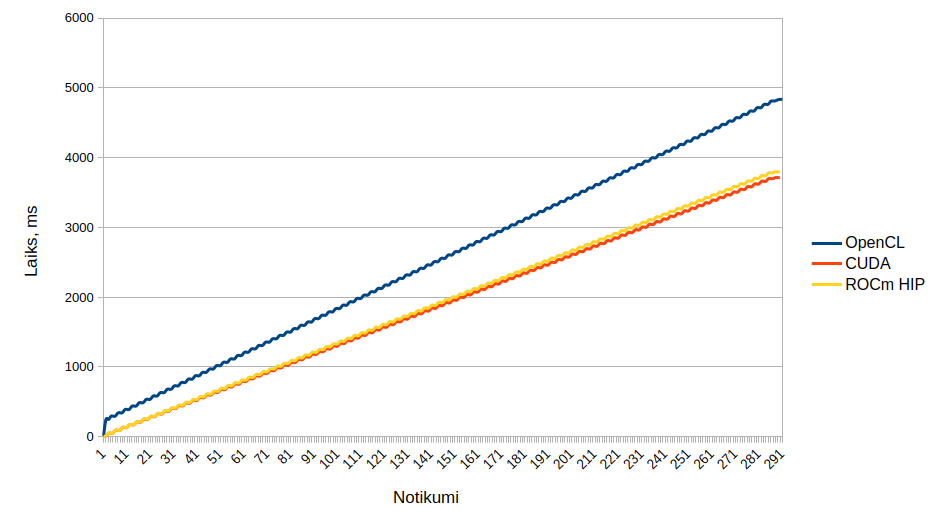
\includegraphics[width=\textwidth]{images/sha256_100m_not_found.png}
    \caption{Paroļu atguvēja izpildes laiki 100m parolēm (parole netika
    atrasta), datu straumes izmērs \( 2^{20} = 1048576\)}
    \label{img:sha256_100m_not_found_cum}
\end{figure}

\begin{figure}[H]
    \centering
    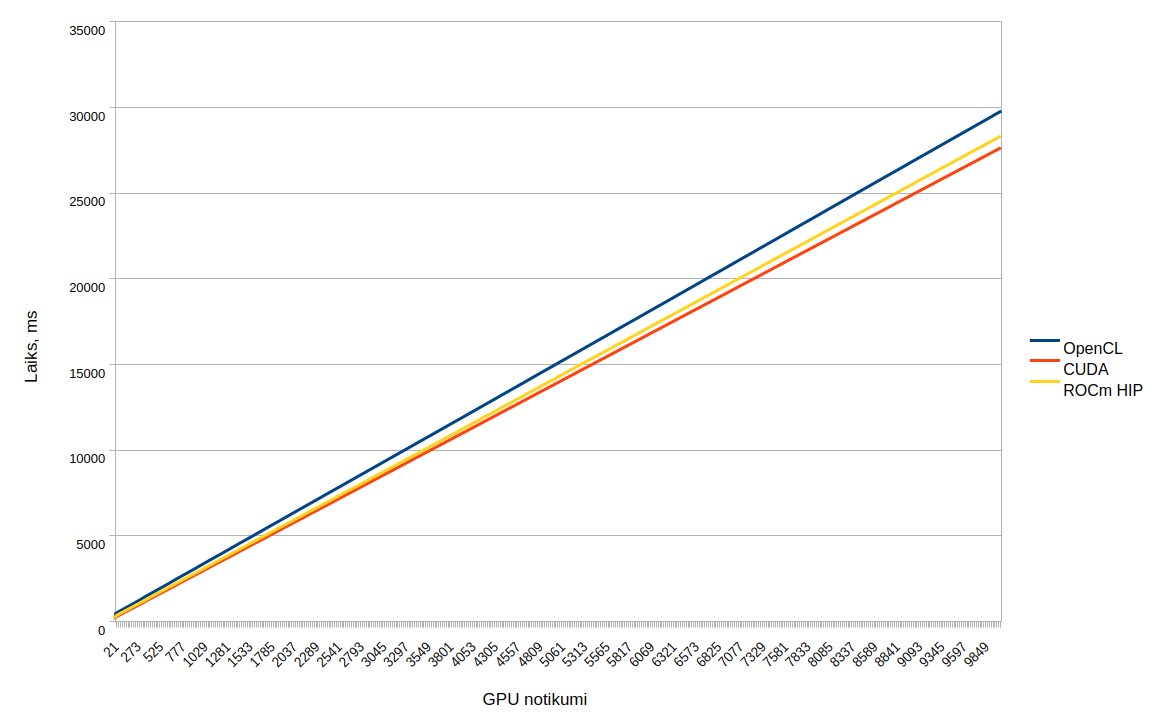
\includegraphics[width=\textwidth]{images/gol_10k_by_10k_10ksteps.png}
    \caption{10000x10000 "Dzīves spēle" ar 10000 soļiem}
    \label{img:gol_10k10k_10k_steps_cum}
\end{figure}

Pēc diagrammām var apstiprināt to, kas jau tika noskaidrots kursa darbā
saistībā ar CUDA un ROCm HIP - ROCm HIP ir neliela virsdarbe, salīdzinot ar
CUDA \cite{kursa-darbs}. Saistībā ar OpenCL platformu katrs notikums, relatīvi
runājot, ir ar daudz lielāku virsdarbi.

Pēc jaunajiem etalonuzdevumiem var secināt, ka vidēji paroles atgūšanas
uzdevumā OpenCL ir par \(30.18\%\) lēnāks nekā CUDA un "Dzīves spēles" uzdevumā
par \(7.71\%\) lēnāks. Bet, salīdzinot HIP ar CUDA, AMD izstrādātā platforma ir
attiecīgi par \(2.25\%\) un \(2.47\%\) lēnāka.

Jāņem vērā, ka šie procenti iekļauj tikai kodolu izpildes laikus abos uzdevumu
gadījumos. Lai gan "Dzīves spēlē" lielākā uzdevuma daļa nodarbojas tikai ar
kodolu izpildi (līdz ar to procentu starpība atbilst diagrammai
\ref{img:gol_10k10k_10k_steps_cum}), paroļu atguvējā starp katra kodola izpildi
notiek datu straumes apstrāde, kas iekļauj datu ielasīšanu no faila,
sagatavošanu GPGPU kodolam un datu pārsūtīšanu uz videokarti, kas aizņem
krietni lielāku laiku nekā paša kodola izpilde.

Ierēķinot kopējos programmu izpildes laikus (failu apstrāde), CUDA bija par
17\% ātrāka nekā ROCm HIP un par 11\% ātrāka nekā OpenCL "Dzīves spēles"
uzdevumā. Bet paroļu atgūšanas uzdevumā CUDA bija par 6\% ātrāka nekā ROCm HIP
un par 30\% ātrāka nekā OpenCL. Abos gadījumos CUDA bija uzvarētāja, bet ROCm
HIP un OpenCL savstarpēji dalīja 2. un 3. vietu. Līdz ar to ir jāņem vērā CPU
puses failu apstrādes virsdarbe, kura var neparedzami ietekmēt mērījumus, jo
pašu kodolu izpildes laiku mērījumi konsekventi sarindo platformas.

Atsevišķi apskatot specifiskus GPGPU notikumus, starp platformām varētu atrast
kodolu izpildes nestabilitāti, tas ir, izpildes laiki varētu būt ļoti dažādi -
ar lielām variācijām. Līdz ar to, ja apskata viena veida laidienu konfigurāciju
mērījumus visās platformās kā izpildes laiku histogrammu, varētu noskaidrot, cik
izkliedēta  ir kodolu izpilde.

Tā kā izmantotās videokartes un CUDA, HIP platformu definētā notikumu
precizitāte ir līdz \(\pm0.5\)\si{\micro\second}, histogrammas "spaiņa" (angļu
val. \textit{Histogram Bin}) platums noteikts kā \(10\)\si{\micro\second} - nav
pārāk šaurs, lai kļūdas dēļ nerastos datu neprecizitātes, un nav pārāk plats,
lai tiktu zaudēta izšķirtspēja \cite{Freedman1981}. No analizējamajiem datiem
izņemti paši pirmie kodolu izpildes mērījumi programmu dzīves ciklā, kuri var
saturēt inicializācijas un kešatmiņas virsdarbes.

Līdzīgs risinājums izmantots paroļu atguvēja žurnālfailu datiem ar papildus
datu filtrēšanu, lai tiktu iekļautas tās kodolu izpildes, kuras pilnībā aizņem
visu datu straumes buferi, pretējā gadījumā kodolu izpildes laiki var būt
neparedzami mainīgi.

\begin{figure}[H]
    \centering
    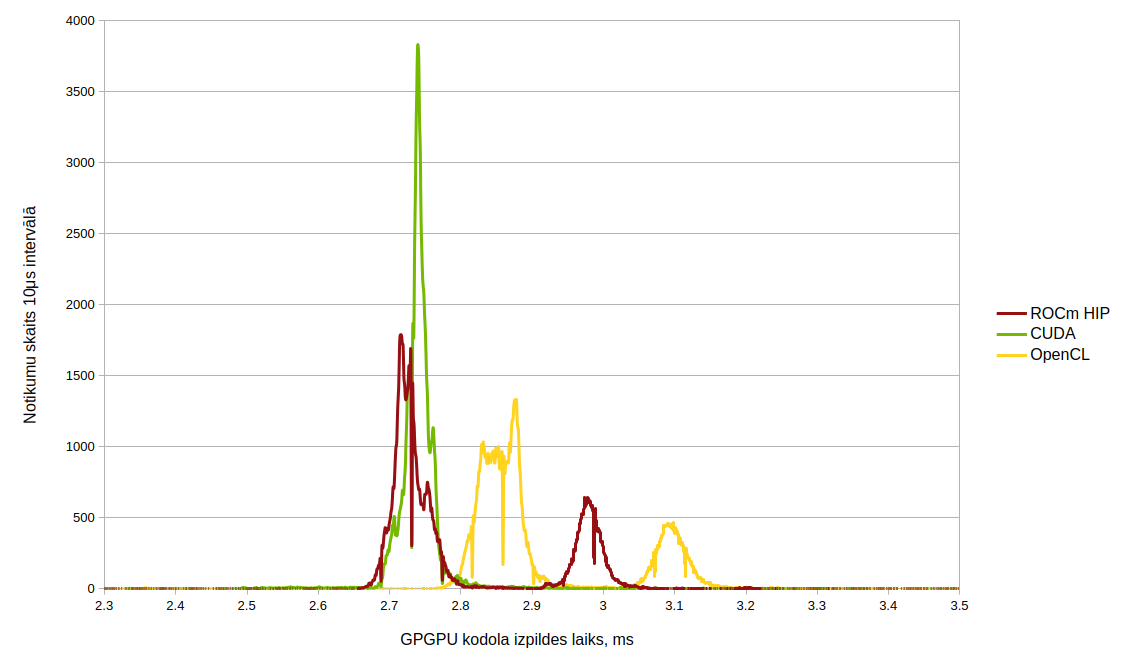
\includegraphics[width=\textwidth]{images/gol_distrib.png}
    \caption{Dzīves spēles kodolu izpildes histogramma (10000x10000 ar 10000 soļiem, 10 laidieni)}
    \label{img:gol_distrib}
\end{figure}


\begin{figure}[H] \centering
    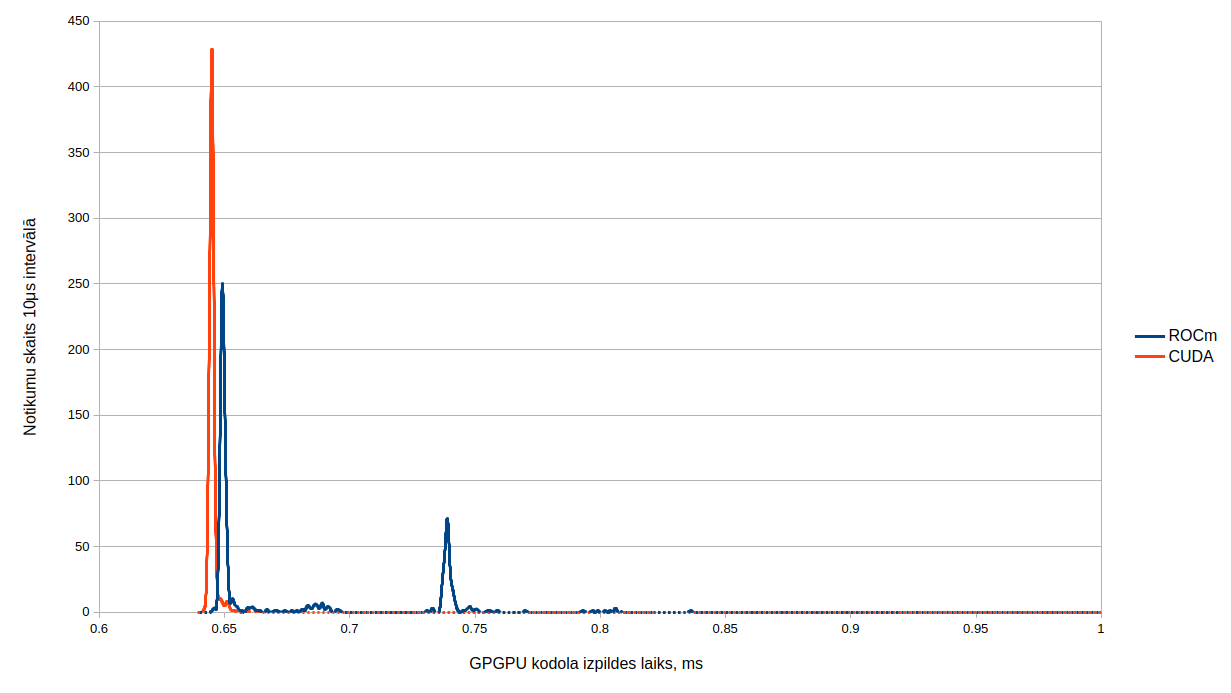
\includegraphics[width=\textwidth]{images/sha_distrib_cuda_rocm.png}
    \caption{Paroļu atguvēja izpildes histogramma CUDA un ROCm platformām (100
    000 000 paroles, 10 laidieni)} \label{img:sha_distrib}
\end{figure}


\begin{figure}[H] \centering
    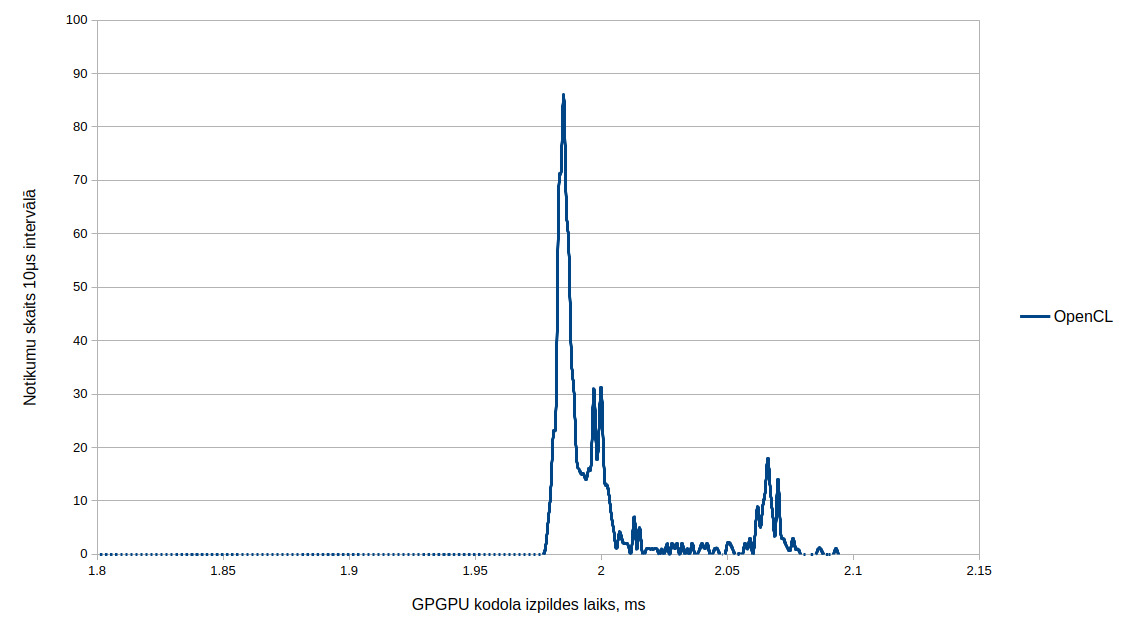
\includegraphics[width=\textwidth]{images/sha_distrib_opencl.png}
    \caption{Paroļu atguvēja izpildes histogramma OpenCL platformai (100 000
    000 paroles, 10 laidieni)} \label{img:sha_distrib_cl}
\end{figure}

Apskatot histogrammu attēlus \ref{img:gol_distrib}, \ref{img:sha_distrib},
\ref{img:sha_distrib_cl}, var redzēt, ka mazākā izkliedētība ir CUDA
platformai. Pieņemot, ka dati veido normālo sadalījumu, tabulās \ref{tab:kern},
\ref{tab:kernel_exec_time_variations_gol} redzamas atbilstošās standartnovirzes
un variācijas.


\begin{table}[H]
    \centering
    \begin{tabular}{lrr}
    \hline
    \textbf{Platforma} & \textbf{Standartnovirze} & \textbf{Variāciju koeficients}\\ \hline
    CUDA    & 0.0015 & 0.0023 \\
    HIP     & 0.0408 & 0.0604  \\
    OpenCL  & 0.0275 & 0.0137 \\
    \hline
    \end{tabular}
    \caption{Platformu paroļu atguvēja kodolu izpildes laiku variācijas}
    \label{tab:kern} 
\end{table}


\begin{table}[H]
    \centering
    \begin{tabular}{lrr}
    \hline
    \textbf{Platforma} & \textbf{Standartnovirze} & \textbf{Variāciju koeficients}\\ \hline
    CUDA    & 0.1613 & 0.0587 \\
    HIP     & 0.1132 & 0.0405  \\
    OpenCL  & 0.1228 & 0.0422 \\
    \hline
    \end{tabular}
    \caption{Platformu "Dzīves spēles" kodolu izpildes laiku variācijas}
    \label{tab:kernel_exec_time_variations_gol} 
\end{table}


Interesants novērojums ir fakts, ka abos uzdevumu risinājumos HIP un OpenCL
izpildes laiku līknes satur divus pīķus ar līdzīgu relatīvo attālumu starp šo
pīķu modām. Datu analīzes laikā tika pieņemta hipotēze, ka šo struktūru veido
GPU aparatūras droselēšana.

Ja tā būtu, tad pie lielas noslodzes, kura ir palielināta HIP un OpenCL
platformām, varēja iestāties aparatūras takts frekvences samazināšana, lai
limitētu sistēmas karšanu. Rezultātā veidojas divi pīķi - viens pie vienas
takts frekvences un viens arī pie otras.

Ja šī hipotēze būtu patiesa, tad varētu secināt, ka videokarte tika pietiekami
noslogota katra HIP un OpenCL laidiena laikā, kas radīja takts frekvences
mazināšanu. Tā kā uzdevumi un darbināmie kodoli ir pietiekami ekvivalenti, tad
palielinātais noslogojums pie pietiekami ekvivalentiem uzdevumiem,
salīdzinājumā ar CUDA, nosaka palielinātu neefektivitāti.

Tālakajā analīzē tika secināts, ka hipotēze ir aplama, jo atkārtotā manuālā
etalonuzdevumu palaišanā netika novērota frekvences mazināšanās, un videokartes
temperatūra nepalielinājās līdz nedrošai robežai. Īstais iemesls tika
atklāts, apskatot secīgus individuālo laidienu kodolu izpildes laikus (skatīt
attēlus \ref{img:consecutive_kernel_exec_gol_cl},
\ref{img:consecutive_kernel_exec_gol_cuda},
\ref{img:consecutive_kernel_exec_gol_hip}).

\begin{figure}[H] \centering
    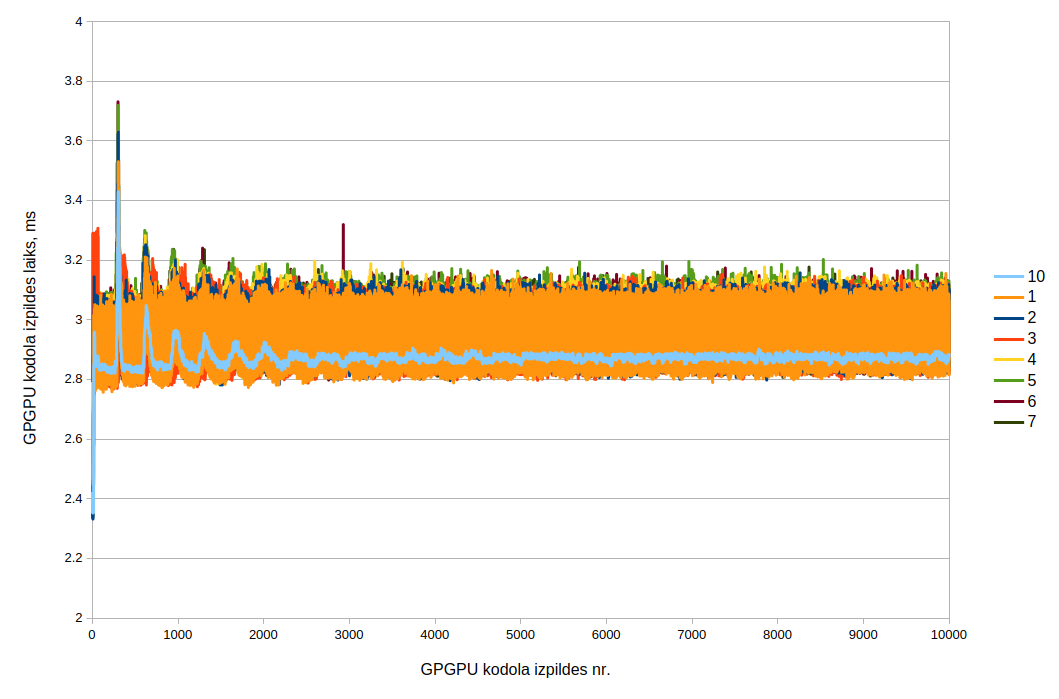
\includegraphics[width=\textwidth]{images/gol_opencl_consecutive_runs_10k_by_10k_10ksteps.png}
    \caption{"Dzīves spēles" secīgo laidienu izpildes laiks OpenCL
    platformā (10000x10000 ar 10000 soļiem)}
    \label{img:consecutive_kernel_exec_gol_cl}
\end{figure}


\begin{figure}[H] \centering
    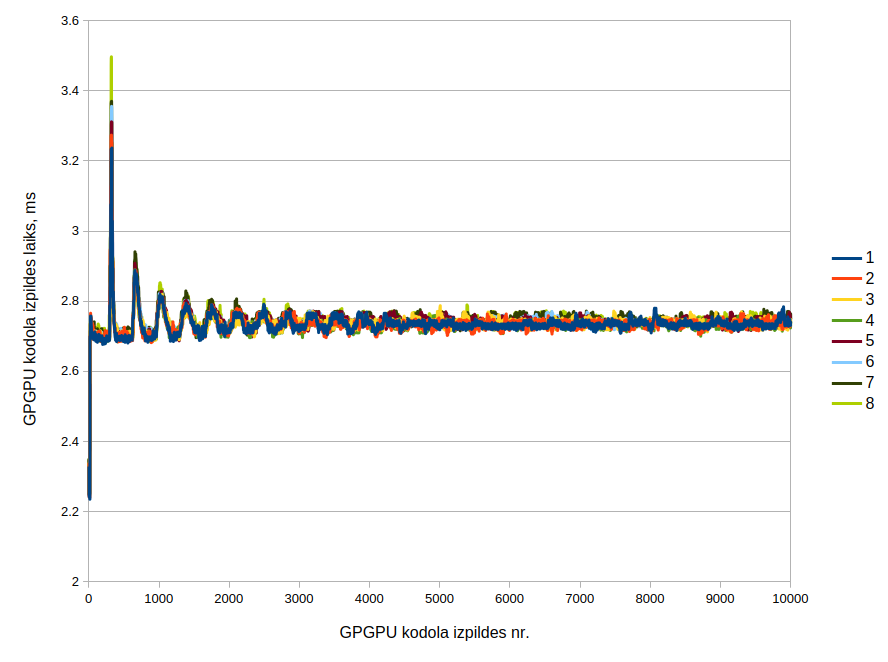
\includegraphics[width=\textwidth]{images/gol_cuda_consecutive_runs_10k_by_10k_10ksteps.png}
    \caption{"Dzīves spēles" secīgo laidienu izpildes laiks CUDA 
    platformā (10000x10000 ar 10000 soļiem)}
    \label{img:consecutive_kernel_exec_gol_cuda}
\end{figure}


\begin{figure}[H] \centering
    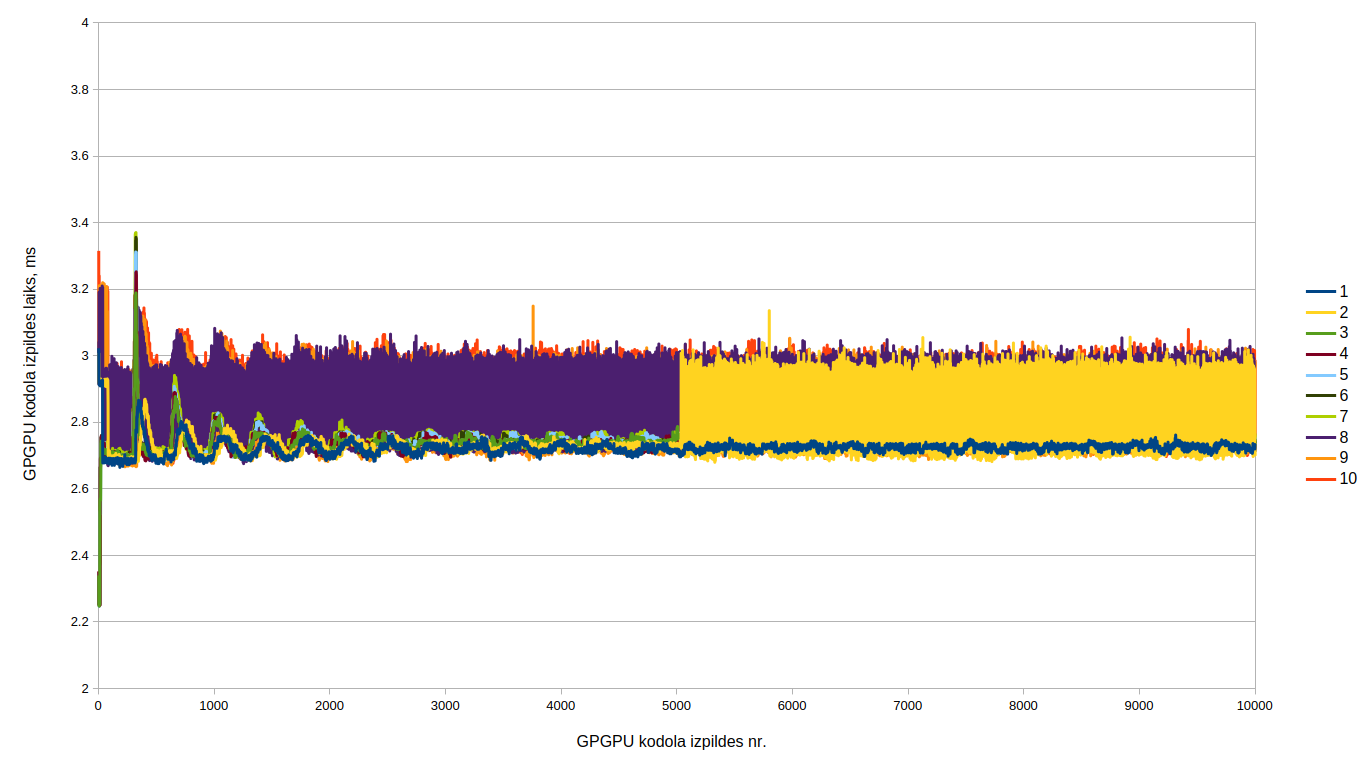
\includegraphics[width=\textwidth]{images/gol_hip_consecutive_runs_10k_by_10k_10ksteps.png}
    \caption{"Dzīves spēles" secīgo laidienu izpildes laiks ROCm HIP
    platformā (10000x10000 ar 10000 soļiem)}
    \label{img:consecutive_kernel_exec_gol_hip}
\end{figure}

Pēc diagrammām var secināt, ka visām platformām ir izteikta sākotnēja
svārstīšanās, kura norimst pēc vidēji 2800 kodolu izpildēm HIP platformai, 4400
CUDA un 2300 OpenCL. Katras platformas individuālie kodolu izpildes laiki ir
7731.7\si{\ms} HIP, 12087.8\si{\ms} CUDA un 6696.1\si{\ms} OpenCL (svārstību
norimšanās laiki citām laidienu konfigurācijām būs citādāki, minētie
ir atbilstoši diagrammās aprakstītajiem). Bet jāņem vērā, ka HIP un OpenCL
vairākos gadījumos ir izteikta nerimstoša svārstīšanās, kura nav raksturīga
nevienam CUDA laidienam starp visām 10000x10000 konfigurācijām. 

Svārstīšanās izskaidrotu vairāku pīķu veidošanos histogrammās, bet pīķu
augstuma dažādība skaidrojama ar faktu, ka HIP un OpenCL nepārtrauktās
svārstības nav sinusoidālas. Ik pa laikam secīgu kodolu izpildes laiki ir
relatīvi līdzīgi, līdz ar to viena veida vērtības, kuras laika ziņā ir mazākas,
parādās izteikti biežāk (skatīt attēlu
\ref{img:consecutive_kernel_exec_gol_hip_cl_sample}).

\begin{figure}[H] \centering
    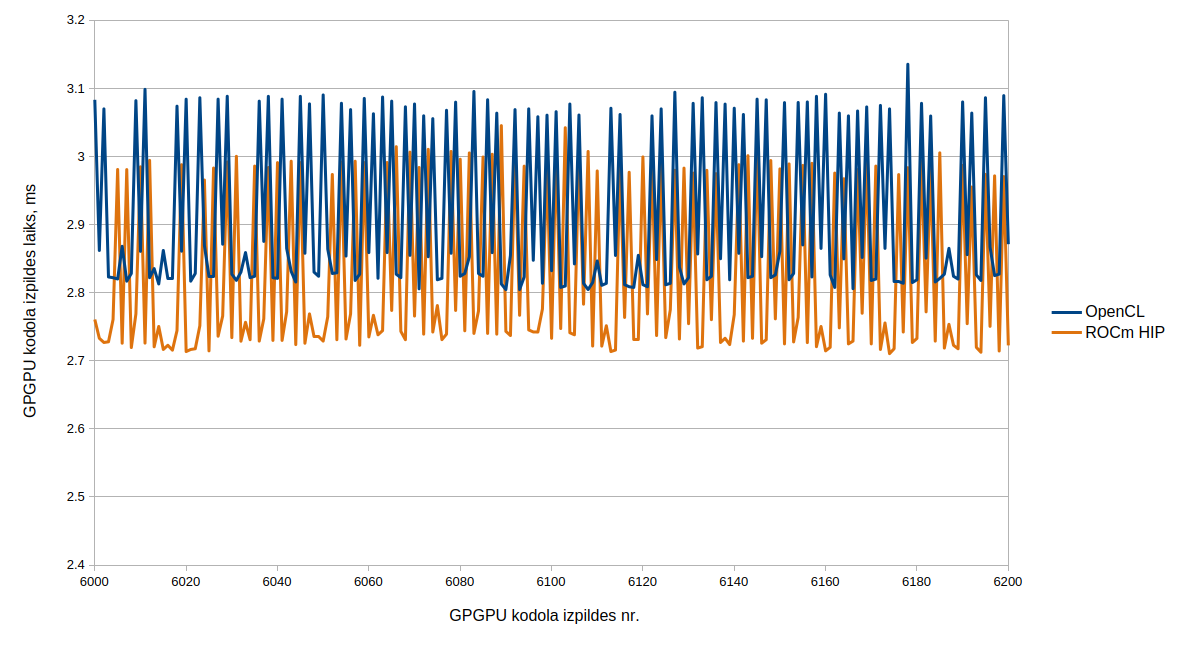
\includegraphics[width=\textwidth]{images/gol_hip_cl_sample_consecutive_runs_10k_by_10k_10ksteps.png}
    \caption{"Dzīves spēles" secīgo laidienu izpildes laiki ROCm HIP un CUDA
    platformā (10000x10000 ar 10000 soļiem)}
    \label{img:consecutive_kernel_exec_gol_hip_cl_sample}
\end{figure}

Līdzīgi ir arī ar paroļu atgūšanas mērījumiem - OpenCL un HIP risinājumiem ir
izteikta nepārtraukta svārstība, kas nav raksturīga CUDA (skatīt attēlus
\ref{img:sha_exec_cl}, \ref{img:sha_exec_cuda}, \ref{img:sha_exec_hip}).

\begin{figure}[H] \centering
    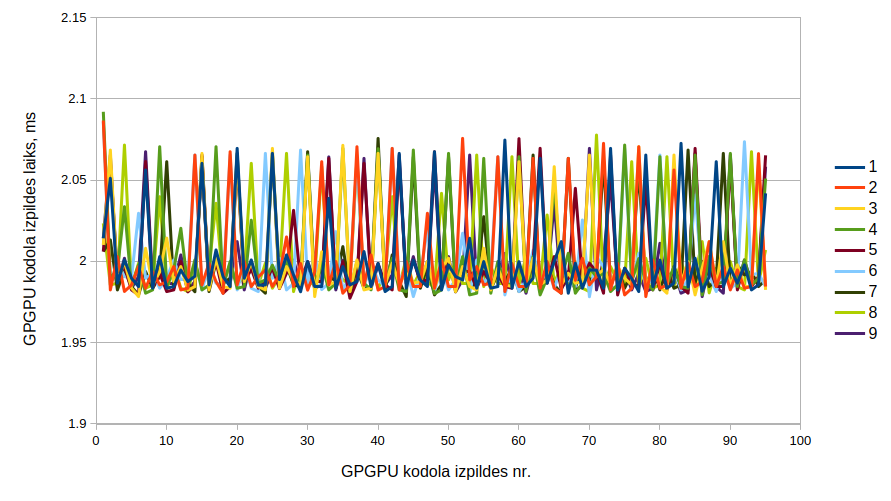
\includegraphics[width=\textwidth]{images/sha_kernel_exec_cl.png}
    \caption{OpenCL paroļu atguvēja kodola izpildes laiki}
    \label{img:sha_exec_cl}
\end{figure}

\begin{figure}[H] \centering
    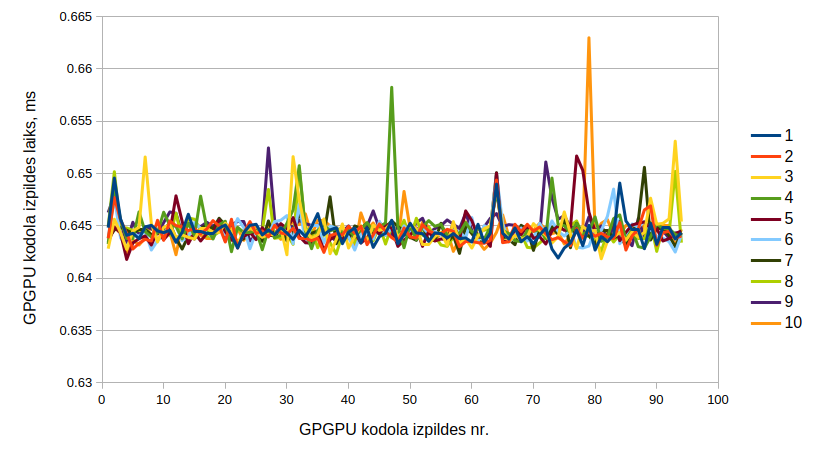
\includegraphics[width=\textwidth]{images/sha_kernel_exec_cuda.png}
    \caption{CUDA paroļu atguvēja kodola izpildes laiki}
    \label{img:sha_exec_cuda}
\end{figure}

\begin{figure}[H] \centering
    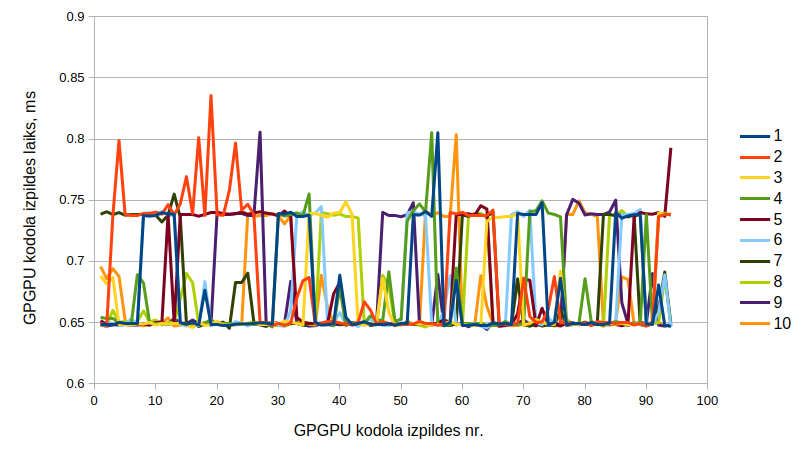
\includegraphics[width=\textwidth]{images/sha_kernel_exec_hip.png}
    \caption{HIP paroļu atguvēja kodola izpildes laiki}
    \label{img:sha_exec_hip}
\end{figure}


Viena GPU puses atšķirība starp uzdevumiem ir nepieciešamība iteratīvi
sagatovot atmiņu un to piepildīt ar straumētajām parolēm paroļu atguvēja
uzdevumā. "Dzīves spēles" uzdevumā šie buferi praktiski netiek aiztikti, jo
izejas režģa buferi var atkārtoti lietot kā ieejas buferi. Paroļu atguvējam
nepieciešams ielasīt jaunus datus visu laiku, tāpēc pirms katras kodola
izpildes tiek sūtīti dati uz VRAM. Šādos mērījumos nav saskatāmas nepārtrauktas
svārstības (skatīt attēlus
\ref{img:sha_buf_creation_cl}, \ref{img:sha_buf_creation_cuda},
\ref{img:sha_buf_creation_hip}).


\begin{figure}[H] \centering
    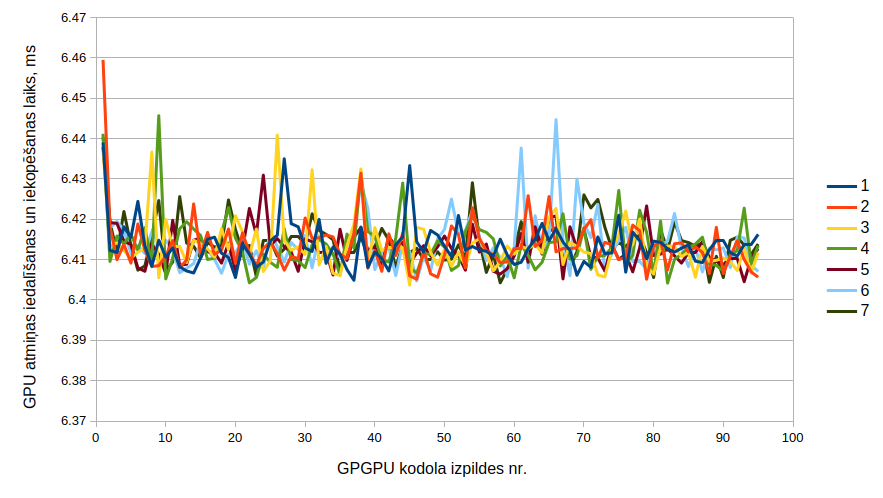
\includegraphics[width=\textwidth]{images/sha_buf_creation_cl.png}
    \caption{OpenCL paroļu atguvēja atmiņas iedalīšana un aizpildīšana}
    \label{img:sha_buf_creation_cl}
\end{figure}


\begin{figure}[H] \centering
    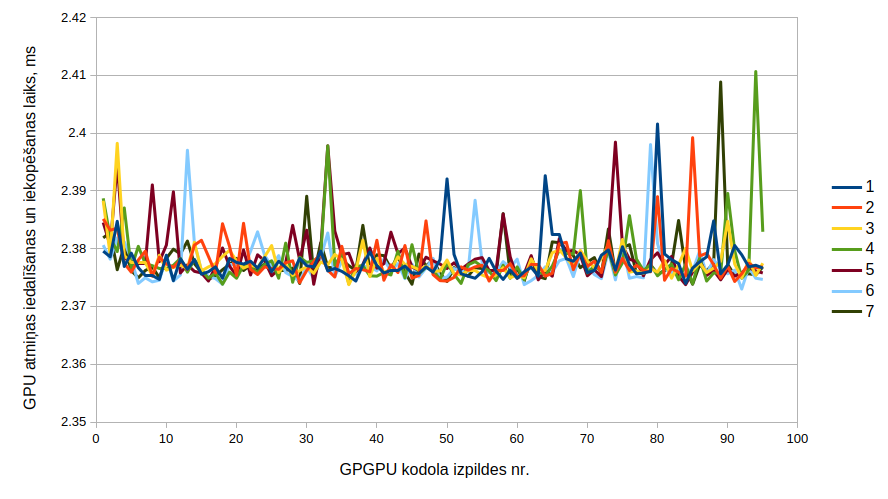
\includegraphics[width=\textwidth]{images/sha_buf_creation_cuda.png}
    \caption{CUDA paroļu atguvēja atmiņas iedalīšana un aizpildīšana}
    \label{img:sha_buf_creation_cuda}
\end{figure}


\begin{figure}[H] \centering
    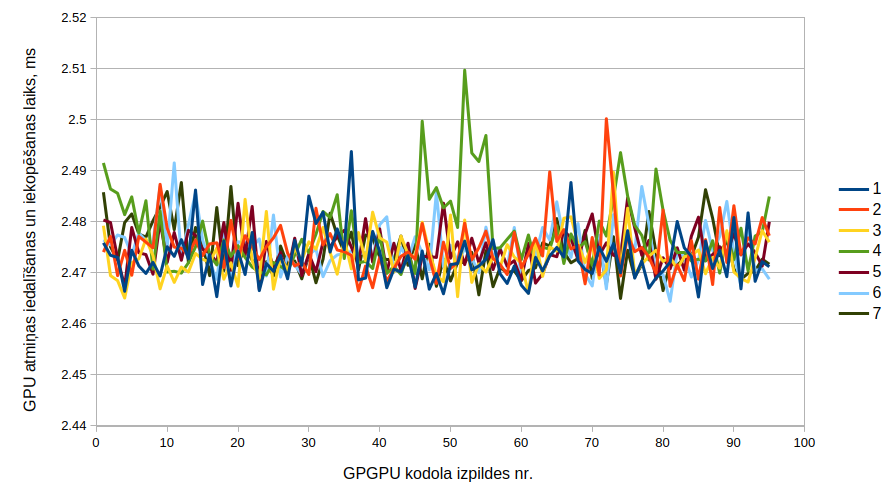
\includegraphics[width=\textwidth]{images/sha_buf_creation_hip.png}
    \caption{ROCm HIP paroļu atguvēja atmiņas iedalīšana un aizpildīšana}
    \label{img:sha_buf_creation_hip}
\end{figure}

Lai gan šķiet, ka izmērītie laiki ir diezgan haotiski un ar lielu amplitūda
visās trijās platformās, jāņem vērā visās atmiņas iedalīšanas diagrammās Y
laika ass solis ir 10\si{\micro\second}, turpretī kodola izpildē tās ir
50\si{\micro\second}. Tabulā \ref{tab:amplitudas} redzams abu mērījumu
amplitūdu salīdzinājums. Pēc to datiem var secināt, ka OpenCL un HIP atmiņas
apstrādes laika variācijai ir mazāka kopējā ietekme uz kodola izpildes laiku,
jo tā variācija ir lielāka. Bet CUDA gadījumā ir redzams pretējais - atmiņas
apstrādes variācijai tomēr ir lielāka ietekme.

\begin{table}[H]
    \centering
    \caption{Paroļu atguvēja GPGPU kodolu izpildes un atmiņas izveides un
    pārsūtīšanas amplitūdu salīdzinājums}
\label{tab:amplitudas}
\begin{tabular}{rrrr}
    Platforma & Kodola izpildes amplitūda, ms & Atmiņas amplitūda, ms& \% \\ \hline
OpenCL & 0.1147 & 0.0558 & 48.65\% \\
CUDA & 0.0212 & 0.0376 & 177.36\% \\
ROCm HIP & 0.1911 & 0.0453 & 23.70\% \\
\hline
\end{tabular}
\end{table}


\begin{center}
    \chapter{Etalonuzdevuma rezultātu līdzvērtība}
\end{center}


\section{Uzticamu etalonuzdevumu izveide}

Lai nodrošinātu, ka etalonuzdevuma rezultāti ir uzticami, tiem jābūt
atkārtojamiem, kā minimums, uz tādas pašas aparatūras un programmatūras.
\cite{reliable-benchmarking}



Kā min viena publikācija \cite{reliable-benchmarking}, mērīt pilno programmas
izpildes laiku var nebūt pietiekoši, piemēram, ar time utilītu, it īpaši
vairākpavedienu scenārijos. Lai gan minētajā pētījumā etalonuzdevumu
sastādīšana apspriesta tīri CPU izpildes kontekstā, vairākpavedienu izpildi un
to ietekmi no I/O darbībām var attiecināt arī priekš GPU.

Kaut kāda programmas izpildes daļa norisināsies uz CPU, un, mērot laikus uz
dažādām aparatūrām (ar uzsvaru uz izteikti atšķirīgu I/O ātrdarbību), var iegūt
neuzticamus rezultātus, jo etalonuzdevuma fokuss nav uz ievades, izvades
ātrumu.

Bakalaura darba autora kursa darbā\cite{kursa-darbs} tika izmantota iepriekš
minētā neieteiktā metode (ar time utilītu mērīts kopējais laiks), bet ņemot
vērā, ka etalonuzdevums tika veikts tikai vienas aparatūras ietvaros, tad
varētu secināt, ka I/O ietekme uz uzticamiem mērījumiem bija minimāla.

Tomēr nevar garantēt, ka, izpildot programmu uz citas aparatūras, varētu iegūt
tādus datus, kas mainītu iegūtos gala secinājumus kursa darbā.

Lai no šādiem riskiem izvairītos, tiks mērīti konkrēti programmas notikumi,
piemēram, kodola kompilēšanas laiks, kodola izpildes laiks, kopējais pavadītais
laiks GPU pusē u.tml.


Līdzīgi nevar iegūt noderīgus mērījumus par atmiņas lietojumu, jo iedalītā atmiņa ne-triviālai programmai mainās laika gaitā.

Tāpēc, kvalitātam etalonuzdevuma uzstadījumam papildus jāsatur:
maksimāli atļautais atmiņas lietojums,
maksimālais programmas izpildes laiks,

Vēl viena prasība ir konsekvents kopējais sistēmas stāvoklis pirms un pēc programmas darbināšanas. Lai to visvieglāk nodrošinātu,
tiks izmantota izolēta OS līmeņa virtuāzijas vide uz Docker\cite{docker-docs-engine} platformas.

Sistēmas stāvokļa neatkarību no CPU un OS kešošanas mehānismiem pavisam atdalīt nav iespējams, tāpēc pirms konkrētas programmas laidienu kopas mērīšanas,
tiks veikts 'iesildošais' laidiens, kura rezultāti netiks ņemti vērā. Tādējādi, mazinot kešatmiņas trāpījumu vai ne-trāpījumu ietekmi uz mērījumiem.

Kopumā definēts šādu uzstādījums, galvenokārt, ņemot vērā izstrādes laikā pieejamo aparatūru:
\begin{itemize}
    \item 16GB RAM,
    \item 6GB VRAM,
    \item gpgpu kodola lokālais grupas izmērs - 256 elementi,
    \item programma darbojas izolētā vidē - Docker konteinerī,
    \item Docker saimnieka operētājsistēma neveic citus relatīvi resurs-intensīvus darbus
\end{itemize}

Priekš Nvidia CUDA un AMD HIP eksistē jau gatavi profilēšanas risinājumi, bet
OpenCL gadījumā nākas pašam apieties ar pieejamajām API funkcijām, līdz ar to
visām programmām jāsatur attiecīgie ekvivalentie GPU notikumu izsaukumi, kuri
tiek vienādi apstrādāti un žurnalēti programmas izpildes laikā. Piemēram, ar
platformu API funkcijām \textit{cudaEventRecord}, \textit{hipEventRecord},
\textit{clGetEventProfilingInfo}.


Datu struktūrām jābūt pietiekami ekvivalentām. To iespējams nodrošināt izmantojot, piemēram, ekvivalentus iebūvētos datu tipus.


Docker konteinera konfigurācija:
\begin{itemize}
    \item Atmiņas ierobežojums - 16GB,
    \item Atmiņas un \textit{swap} atmiņas ierobežojus - 16GB,
    \item Apstrādes failu piekļuvei no OS montēts sējums (angļu val. \textit{volume}) konteinera /data direktorijā
\end{itemize}






\begin{center}
    \chapter{Uzdevumu definīcija un realizācija}
\end{center}

HIP risinājumiem par pamatu izmantots AMD ROCm izveidotais Docker fails \cite{hip-lib-docker}
kas definē gatavu izstrādes vidi tālākam darbam ar ROCm vai CUDA.



Situācijās kad kāda attiecīga OpenCL API funkcija nepiedāvā profilēšanas informāciju, CPU pusē funkcijas izpildes laiks mērāms ar chrono - steady clock 
Šādās situācijās arī CUDA un ROCm attiecīgās funkcijas izpildes laiks mērāms šādi, pat ja pieejama profilēšanas informācija, kas būtu precīzāka.
Šādi darīts, lai lieku ietekmi uz rezultātiem neradītu chrono virsdarbe vai profilēšanas virsdarbe.

GPGPU arhitektūra un programmēšana
\begin{center}
\chapter{GPGPU arhitektūra un programmēšana}
\end{center}

Procesi, kas izmanto GPU resursus, tipiski iedala atmiņu un sagatavo datus uz CPU, un tad nodod darbu
grafiskajam procesoram. Atmiņas iedalīšanas varianti ir stipri atkarīgi no veicamā uzdevuma un, būtiskāk, no
pieejamā GPU arhitektūras.

Vecākās videokartēs atmiņas iedalīšanu strikti veica CPU un to atmiņas ir pavisam atdalītas 
(RAM un VRAM - Video RAM). Modernāki risinājumi spējīgi pielietot vienotu
atmiņas apgabalu (CPU un GPU abi var piekļūt viens otra atmiņai), piemēram, Nvidia kartes sākot ar Pascal
mikroarhitektūru \cite{nvidia_tesla_p100}. Rezultātā programmētājam nav jāpārvalda,
kuras adreses ir centrālā un kuras grafiskā procesora. Vēl arī jāapsver, vai ir iespēja pa tiešo no GPU
iedalīt atmiņu, vai to darīs tikai CPU.

Protams, noteiktus abstrakcijas slāņus zemāk, procesoru atmiņas tomēr dzīvo dažādās vietās un nav apvienojami,
izņemot procesorus, kuros CPU un GPU dzīvo vienā čipā (integrētās videokartes).

Uz GPU izpildāmā programma tiek saukta par kodolu (no angļu val. \textit{kernel}), un no CPU ar draiveru
palīdzību tiek nodots:
\begin{itemize}
    \item uz GPU pavedieniem izpildāmais kodols,
    \item pavedienu skaits,
    \item kodola funkcijas argumenti (visbiežāk tās būs apstrādājamo datu atmiņas adreses - rādītāji).
\end{itemize}

Jāpārveido, lai nav grāmatas tulkojums:    GPU sastāv no daudziem kodoliem un katrs kodols izpilda
SIMT (\textit{Single instruction, multiple threads}) modelim atbilstošu iedoto izpildāmo kodolu




Derētu tad minēt šādas lietas
\begin{itemize}
   \item Augsta darbu paralelizācija lielo kodolu skaitu dēļ
   \item Īpašas instrukcijas konkrētu datu apstrādei
   \item Darbus nodod procesors (kaut kā īsti nezinu kā) GPU un GPU izmet atpakaļ rezultātu vai prasīto uzzīmē uz ekrāna
   \item Darbus var nodot GPU caur saskarnēm kā Nvidia CUDA vai AMD ROCm
\end{itemize}

SIMT kodoli - single instruction, multiple threads. Sadalās SIMT frontendā un SIMD (multiple data) backendā

SIMT steks, lai atbilstītu zarošanos

SIMT deadlock - paveidiens gaida uz atomicCAS, tālāk neies kamēr neizpildīs (while (!atomicCAS) ...), kad to dara vairāki paveidieni, tad var notikt deadlock

\begin{center}
\chapter{Platformu salīdzinājums}
\end{center}
Lai piesaistītu GPU programmētājus, AMD jau no sākuma dizainēja ROCm, lai tā līdzinātos CUDA. Protams,
abas platformas ir paradzētas GPU programmēšanai un apakšējā videokaršu arhitektūra nebūs tik atšķirīga.
Galvenā atšķirība, neskaitot platformu mērķa grafiskos procesorus, ir fakts, ka atšķirībā no CUDA, kura
ir slēgtā, ROCm ir atklātā pirmkoda programmatūra, līdz ar to, ja nepieciešams, visu programmatūras saturu 
var izpētīt, modificiēt, kompilēt pats, kā arī dot savu pienesumu gan dokumentācijā, gan kodā.\cite{what_is_ROCM}

ROCm dokumentācija ir ar savām problēmām, piemēram, lai atrastu instalāciju nākas diezgan dziļi meklēt
un 'lēkāt' starp lapām, lai atrastu konkrēto instalācijas failu. Instalācijas pamācības un lejupielādes
lapas ir diezgan sadalītas. CUDA šis process ir vienkāršāks, kā arī CUDA ir pastāvējusi daudz ilgāku
laiku, līdz ar to pieejamā literatūra, forumu diskusiju skaits ārpus oficiālajām dokumentācijām ir daudz 
lielāks nekā priekš ROCm.

ROCm satur vairākas programmas, bibliotēkas un ietvarus dažādiem darbiem ar augstas veiktspējas,
paralelizācijas skaitļošanu, bet konkrētais C++ API priekš GPU programēšanas ir HIP (no angļu val.
\textit{Heterogeneous-computing Interface for Portability}).\cite{HIP_docs}

Noteiktas HIP dizaina izvēles ir tieši aizņemtas no CUDA, lai CUDA vidē pieredzējušajiem
izstrādātājiem pāriet uz ROCm būtu vieglāk. Piemēram, C++ dekoratori, kuri norāda vai funkcija ir CPU
vai GPU, vai GPU kodola funkcija ir vienādi (skatīt  izdruku \ref{lst:cuda_hip_fn_decorators}).

\begin{lstlisting}[caption={CUDA un HIP funkciju definīciju salīdzinājums},
  label=lst:cuda_hip_fn_decorators,
  captionpos=t
]
// CUDA:
__host__ myCpuFunction() {/*...*/}
__device__ myGpuFunction() {/*...*/}
__global__ kernel() {}

// HIP:
__host__ myCpuFunction() {/*...*/}
__device__ myGpuFunction() {/*...*/}
__global__ kernel() {/*...*/}
\end{lstlisting}

HIP ir diezgan liels atbalsts ne tikai AMD videokartēm, bet arī Nvidia. Tas iespējams tāpēc, ka 
daudzas HIP saskarnes ir CUDA savietojamas, piemēram, GPU matemātisko funckiju API, tās saturošās funkcijas
ir tieši atbilstošas CUDA funkcijām.\cite{HIP_math_API,CUDA_math_API}

Kompilēšanas līmenī šis atbalsts ir iespējams, jo HIP izmanto kompilatoru draiveri 'hipcc', kurš,
atkarībā no platformas, veiks pirms-apstrādi un izsauks attiecīgo kompilatoru -
AMD videokartes gadījumā 'amdclang++' un Nvidia CUDA - 'nvcc'. \cite{HIP_compilers}.

Tā kā varētu interpretēt, ka CUDA ir tieša apakškopa ROCM un HIP platformai, bet tomēr pilnīgs atbalsts
visām CUDA funkcijām nav pieejams.



Tā kā, rakstot CUDA kodu, arī tiek izmantots tas pats 'nvcc' kompilators, ROCm piedāvā utilītu
pirmkoda migrēšanai - 'HIPIFY'. \cite{HIPIFY_github}

Potenciāls mīnuss HIP saistītām utilītām un bibliotēkam ir fakts, ka vairākām nav pieejama
"\textit{out of the box}" instalācija. Ir nepieciešamība kompilēt pirmkodu pašam, šo papildus soli
sarežģī atkarīgo pakešu pārvaldīšana. Windows gadījumā arī rodas sarežģījumi, jo ROCm utilītu noklusētā vide
ir Linux un visa ROCm izmantotais kompilators ir Clang/LLVM, kam uz Windows ir nepieciešama papildus 
konfigurēšana.
Piemērs šādai utilītai ir "HIPIFY", ar kuru iespējams pārveidot CUDA pirmkodu uz HIP. \cite{HIPIFY_github}

Tā kā CUDA ir slēgtā pirmkoda, tad, protams, visa programmatūra un rīki pieejami caur instalācijām un
rezultātā šis process ir daudz vienkāršāks.

Lai gan HIP atbalsta ir diezgan liels ierobežojums atbalstītajām videokartēm




ROCm paradzētā vide ir Linux, bet CUDA tā ir Windows. ROCm dokumentācijā, kur nepieciešams darbs ar komandrindas rīkiem, pamācības ir tikai Linux operētājsistēmai. CUDA gadījumā problēmas rodas jau instalācījas brīdī darbā ar Linux, jo nepieciešamas papildus darbības, konfigurācijas atkarībā no distributīva, izmantotā pakotņu pārvaldnieka sistēmas.

Atšķirībā no AMD, CUDA neizplata informāciju par savām videokartēm un tā kā Linux pats par sevi ir atklātā
pirmkoda programmatūra, tā nenāk ar Nvidia draiveriem. Tomēr projekts nouveau ar reversēs inženierijas
metodēm cenšas piedāvāt atklātā pirmkoda draiverus nvidia videokartēm
% https://en.wikipedia.org/wiki/Nouveau_(software)

Bet, lai izmantotu CUDA šis risinājums neder, jebkurā gadījumā nāksies overridot visus ne-Nvidia izlaistus draiverus. Linus |TOrvalds par arī ir izteicies, ka nosoda šādu kompānijas politiku.


% https://docs.nvidia.com/cuda/cuda-installation-guide-linux/index.html



ROCm nav iekļauts populārākajās pakotņu pārvaldnieku sistēmās, lai gan ar automātisko instalāciju 
tiek iekļauts visa nepieciešamā programatūrā darbam ar ROCm programmām, problēmas rodas saskarnē ar
CUDA, jo nākas atrisināt atkarību problēmas. Noklusēti tiks meklēta cuda atkarība distributīva izmantotajā
pārvaldniekā, piemēram, Ubuntu "apt". Bet, šī atkarība satur tikai CUDA draiverus, nevis 
izstrādes rīkus, lai veiktu darbu ar CUDA Toolkit. 

Līdz ar to ir manuāli jāatrisina neatbilstošas pakotņu atkarības.


% https://github.com/ROCm/HIP/issues/820 - kā atrisināt cuda dependency




Kopumā AMD mērķis ar ROCm, atbalstot konkurent-kompāniju, ir sniegt gala lietotājiem, izstrādātājiem
vieglāku pārēju uz AMD platformu un videokartēm. Uzturot funkcionalitāti platform-neatkarīgu un
programmatūru rakstot HIP platformā, izstrādātāji ir spējīgi atbalstīt abu platformu videokartes.

Rezultātā kompānijas un gala lietotāji, sastādot datoru, serveru specifikāciju, varētu neuztraukties
par platform-atkarību, jo uzņēmumam svarīgā programmatūra, piemēram, mašīnmācīšanās bibliotēkas
strādātu bez problēmām gan uz Nvidia, gan AMD videokartēm.

AMD gadījumā, protams, ka labāka situācija būtu, ka tiktu izvēlēta viņu ražota videokarte. Un šādā teorētiskā
scenārijā tāds arī būtu iznākums, jo aptuveni vienādas specifikācijas videokartes starp abiem ražotājiem
ir ar lielu cenas starpību.

TABULA AR SPECIEM UN CENU


Bet, tā kā CUDA parādījās pirmā, kļuva par industrijas standartu un agrāk citu risinājumu nebija, 
mūsdienās plaši lietota programmatūra ir rakstīta uz CUDA. Piemēram, mašīnmācīšanās bibliotēka TensorFlow. \cite{tensorflow_github}

Migrēšana lielos projektos tomēr nav tik vienkāršs process, un ar šobrīdējo lielo AI pieprasījumu 


\chapter{Uzdevums}

Praktiskai platformu salīdzināšanai tomēr būtu nepieciešama videokarte.
Darba izstrādes laikā bija pieejams portatīvais dators ar:
\begin{itemize}
  \item AMD Ryzen 5600H procesoru ar Radeon Graphics integrēto videokarti
  \item Nvidia GeForce RTX 3060 Laptop ārējo videokarti
\end{itemize}

Lai gan it kā viena datora ietvaros būtu pieejamas gan Nvidia, gan AMD videokartes, diemžēl
integrētajai Radeon Graphics kartei nav ROCm atbalsts, kā arī HIP nav oficiāls atbalsts 
Nvidia videokārtēm uz Windows, tikai Linux. \textcolor{red}{Tāpēc par pamata platformu analīzē tiks izmantota CUDA.}

Iespējams risinājums ir WSL - \textit{Windows Subsystem for Linux}, ar kuru iespējams izmantot
Linux paredzētās programmas uz Windows. Gan CUDA, gan ROCm ir atbalsts un pamācības kā sakonfigurēt 
šīs platformas darbam uz WSL.\cite{nvidia_wsl_guide,rocm_wsl_guide}







Bet ņemot vērā, ka HIP atbalsta arī CUDA, būs iespējams apskatīt HIP iespējas uz Nvidia videokartes.

Jāizvēlas tāds uzdevums, kuru iespējams 'augsti' paralelizēt, tas ir, sadalīt uzdevumu daudzos mazos gabalos (vēlams skaitā >= 1 miljons),
lai būtu pievienotā vērtība (ātrdarbība) to pildīt uz GPU, ņemot vērā papildus darbu un nepieciešamās zināšanas, lai ieviestu GPU risinājumu.

Relatīvi vienkāršs, bet pietiekams uzdevums, lai parādītu ietvaru atšķirības un vispārīgi atšķirīgās
paradigmas starp CPU un GPU programmēšanu būtu paroļu lauzējs.

Nobriedušāki paroļi lauzēji, jeb precīzāk - paroļu atkopēji kā HashCat ir spējīgi ņemt vērā vairākas paroļu
variācijas, maskas, faktus, ka parole, piemēram, iesākusies ar "123" un citas sarežģītākas potenciālo paroļu
iegūšanas metodes. Demonstrācijas vajadzībām pietiktu izstrādāt pašu 'kodolu', kas, ar jau saņemtu
iespējamo paroļu sarakstu, tās pārbaudīs.


Tātad jāizstrādā programma, kas ņemot vērā ieejas failu ar potenciālajām parolēm, no kādas paroles
jaucējvērtības spētu noskaidrot 'hešoto' paroli.
Uzdevumu būtu vērts risināt uz GPU, jo pie liela paroļu skaita, katrs GPU kodols varētu rēķināt savas
paroles jaucējvērtību un pārbaudīt to pret uzlaužamo.

\section{Izstrādājamās programmas definīcija}
Programma ir domāta kā komandrindas utilīta ar CLI argumentiem:
\begin{itemize}
  \item testu palaišanais arguments
  \item ievades faila ceļš,
  \item paroles jaucējvērtība.
\end{itemize}

Apstrādājamais fails saturēs potenciālās paroles, katra savā rindā, kurām tiks izrēķināta jaucējvērtība un
salīdzināta pret doto. Izmantojamais jaukšanas algoritms - SHA256. Jaucējvērtību rēķināšana un salīdzināšana
jārealizē izpildei uz GPU.

SHA256 izvēlēts tā tīri tā popularitātes un relatīvi ātrās izpildes dēļ, paroles uzlaušanas demonstrācijas
vajadzībām ar šo pietiek, nepieciešamības gadījumā iespējams ieviest citu jaukšanas algoritmu un aizstāt
ar esošo.


Programmu iespējams palaist ar:
\begin{itemize}
  \item \texttt{\$ pwCracker --test}, lai vispārīgi pārbaudītu programmas darbību pret zināmām jaucējvērtībām
  un to attiecīgajiem ziņojumiem, kā arī, lai pārbaudītu GPU kodola programmas darbību, platformas
  pieejamību uz šī datora apartūras
  \item \texttt{\$ pwCracker <paroļu faila ceļs> <paroles hash vērtība>}, lai veiktu galveno programmas izpildi
\end{itemize}


\subsection{CUDA risinājums}

Lai gan CUDA ir domāta izstrādei uz C++, izpildāmais kods uz GPU ir ar saviem ierobežojumiem, kas neļauj pielietot C++ standarta bibliotēkas funkcijas, jo tās iekš 'CUDA device code' nav implementētas.
Vai nu tāpēc, ka kāda konkrēta funkcija ir visparīgi reti lietota, vai tā nav īsti paredzēta lietošanai iekš GPU.

Piemēram, nav pieejamas std::string, std::vector struktūras, jo tās dinamiski iedala atmiņu, kas darbībā iekš CUDA kerneļa būtu ļoti lēna darbība.
Tā kā paroles par nelaimi ir simbolu virknes, tad tās nāksies apstrādāt C stilā (char*), vai arī kā baitu masīvus (uint8\_t*).

Izstrādē ir jāvelta arī palielināta uzmanība datu struktūrām, to izvietojumam atmiņā, piemēram,
problēma kā glabāt pārbaudāmo paroļu sarakstu. Naivais risinājums būtu masīvs ar adresēm, kuras norāda uz pirmo simbolu konkrētās paroles simbolu virknē.

Problēma šajā risinājumā ir, ka netiek nodrošināta atmiņas blakusnodalīšana, tas ir, vienā nepārtrauktā atmiņas
apgabalā, jo konkrētā parole var teorētiski atrasties jebkur, paroles savstarpēji nav obligāti viena otrai
blakus. Līdz ar to varētu rasties lēndarbība no konkrētā pavediena izpildes kodolā - katrs pavediens savu
paroli meklētu teorētiski patvaļīgā vietā, kas var radīt kešatmiņas netrāpījumus.


Arī datu kopēšanas uz GPU atmiņu būs lēna, nāksies izmantot vairākas cudaMemcpy instrukcijas, katrai parolei.

Labāks risinājums ir izmantot nepārtrauktu paroļu buferi un katrai parolei fiksēt garumu, tām liekot galā 
nuļļu papildinājumus.


Jāņem vērā arī definētie kerneļa bloku un pavedienu skaiti ..

A reasonable minimum target is to launch a total number of threads of at least of SM * 2048.

https://forums.developer.nvidia.com/t/cuda-sha256-calculations-improvements/56757/4

These should be split between blocks with usually something in the range of 128,256, or 512 threads per block. It might be that 1024 threads per block is “OK”, it just requires some analysis to confirm.

Your GTX970 has 13 SMs, so target 13*2048 = 26K threads, ballpark, minimum. If you put 1024 threads per block, that would be 26 blocks. I’m not saying I know how to transform your code from 4 blocks to 26, but that is a reasonable performance goal, to maximize throughput.

\begin{lstlisting}
__global__ void kernel(
    const cuda::std::uint8_t *passwords,
    const int *pwLengths,
    int pwCount,
    cuda::std::uint64_t maxPwLength,
    const cuda::std::uint8_t *targetHash,
    int *resultIndex
)
{
    int idx = blockIdx.x * blockDim.x +threadIdx.x;

    if(idx >= pwCount)
    {
        return;
    }

    const cuda::std::uint8_t *password = passwords + (idx * maxPwLength);
    int pwLength = pwLengths[idx];

    cuda::std::uint8_t hash[32];


    sha256(password, pwLength, hash);

    // ja hashi sakrīt, tad ierakstām paroles indeksu iekš 'resultIndex',
    // tā kā tā mainīgā adrese atrodas device kopīgajā atmiņā, jālieto atomiska funkcija
    if(compareHashes(targetHash, hash))
    {
        // ja resultIndex glabājas vērtība -1, tad aizstāj to ar idx
        // ar šo tiek arī reizē nodrošināts, ka ja kāds pavediens vēlāk tomēr nonāk līdz šim stāvoklim,
        // tad modifikācija netiks veikta, jo tajā brīdī jau 'resultIndex' != -1
        atomicCAS((unsigned int*)resultIndex, -1, (unsigned int)idx);
    }
}
\end{lstlisting}


\texttt{nvcc -O2 kernel.cu -o main.exe}

\subsection{Portēšana uz HIP caur WSL 2}

\subsection{Analīze un secinājumi}

Ir jāpievērš uzmanība mērķa videokartei un mikroarhitektūrai, jo izstrādājot programmu uz personīgā datora 
ar RTX 3060 videokarti bija pieejamas funkijas, kuras testējot uz cita datora ar Quattro sērījas videokarti,
programma nestrādāja.

Ir situācijas, kad šo problēmu var atrisināt, kompilācijas brīdī definējot mērķa arhitektūras, bet,
ja izmantota kāda konkrēta funkcionalitāte, kura vienkārši nav pieejama uz mērķa, programma nestrādās.


Veiktspējas metrikas

\textbf{Vēl ir jāņem vērā virsdarbe, kopējot datus no iekārtas uz CPU un atpakaļ, šāda darbība ir relatīvi dārga}

\chapter{Platformneatkarīgi risinājumi}
ZLUDA, OpenCL


\cleardoublepage
\phantomsection
\addcontentsline{toc}{chapter}{Bibliogrāfija}
\printbibliography

\newpage
\chapter*{Pielikumi}
\addcontentsline{toc}{chapter}{Pielikumi}


Ja darbam nepieciešams, dažādus palīgmateriālus var ievietot pielikumā. Tajā
parasti iekļauj aprēķinu starprezultātus, ilustrācijas, anketu paraugus, kartes, aparātu un ierīču aprakstus u. c.


%dokumentācijas lapa
% autoram/ei izskatīt, nomainīt locījumu vārdiem
\newpage
\thispagestyle{empty}
\makeatletter
{\setstretch{2.0}
\noindent
\degree \ "\@title" izstrādāts LU Datorikas fakultātē.
\newline
\newline
\noindent
Ar savu parakstu apliecinu, ka pētījums veikts patstāvīgi, izmantoti tikai tajā norādītie informācijas avoti.
\newline
\newline
\noindent
Autors: \@author \space \rule{30mm}{0.2mm}
\newline
\newline
\newline
\noindent
Rekomendēju/nerekomendēju darbu aizstāvēšanai (nevajadzīgo izsvītrot)
\newline
\newline
\noindent 
\supervisor \space \rule{30mm}{0.2mm}
\newline
\newline
\newline
\newline
\newline
\noindent 
Darbs iesniegts Datorikas fakultātē
\newline
\newline
\noindent 
Dekāna pilnvarotā persona:
\newline
\newline
\newline
\newline
\noindent 
Darbs aizstāvēts kursa darbu komisijas sēdē
\newline
\newline
\newline
\newline
\newline
\noindent 
Komisija:
}
\makeatother

\end{document}
